\documentclass[UTF8,11pt,handout]{beamer}

\usepackage[utf8]{inputenc}
\usepackage{latexsym}
\usepackage[T1]{fontenc}
\usepackage{lmodern}
\usepackage[english]{babel}
\usepackage{amsmath}
\usepackage{amsfonts}
\usepackage{amssymb}
\usepackage{graphicx}
\usepackage{tikz}
\usetikzlibrary{matrix,shapes,arrows,positioning,fit,backgrounds,calc}
\usepackage{overpic}
\usepackage[]{algorithm}
\usepackage[]{algpseudocode} % noend
\usepackage[most]{tcolorbox}
\usepackage{ulem}
\usepackage{fancybox}
\usetikzlibrary{decorations.pathreplacing}
\usetheme{Eastlansing}
\newcommand{\fallingfactorial}[1]{%
	^{\underline{#1}}%
}
\mode<presentation>
\begin{document}
	\author{MA Jun}
	\title{Problem Solving}
	\subtitle{2-9 Sorting and Selection}
	\logo{
\includegraphics[width=0.05\textwidth]{figs/ICS_LOGO_left.png}}
	\institute{Institute of Computer Software}
	%\date{March 31, 2020}
	%\subject{}
	%\setbeamercovered{transparent}
	%\setbeamertemplate{navigation symbols}{}
\begin{frame}[plain]
	\maketitle
\end{frame}
\begin{frame}           %生成目录页,目录太长时加选项[shrink]
	\addtocounter{framenumber}{-2}%---------位置放在beginframe之后,不然无效
	\frametitle{Contents}
	\thispagestyle{empty}
	\tableofcontents[hideallsubsections]
\end{frame}
\AtBeginSection[]{
	\begin{frame}           %生成目录页,目录太长时加选项[shrink]
		\addtocounter{framenumber}{-1}%---------位置放在beginframe之后,不然无效
		\frametitle{Contents}
		\thispagestyle{empty}
		\tableofcontents[currentsection]
	\end{frame}
}
\section{Sorting}
\subsection{Quicksort}
\begin{frame}[t]
	\frametitle{Quicksort}
	\question{}{What is the \textcolor{red}{\textbf{KEY}} idea of Quicksort?}
		\begin{center}
			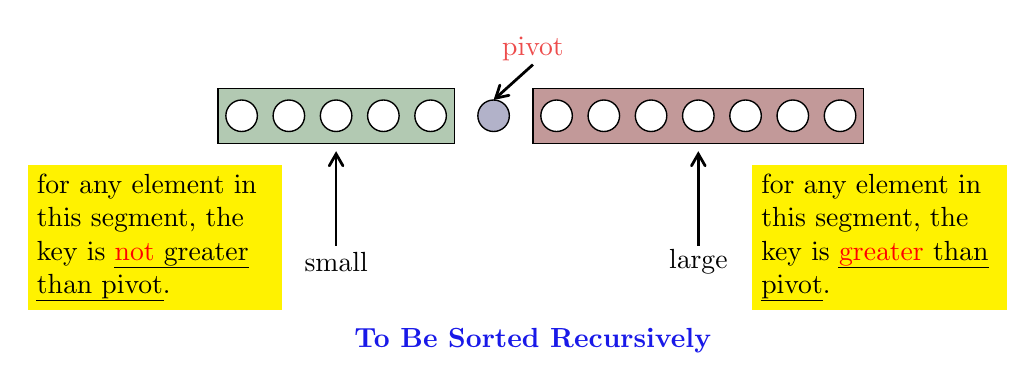
\begin{tikzpicture}
			\pause{
				\filldraw [fill=green!30!black!30,draw=black,line width=0.5pt] (0,0) rectangle (3,0.7); 
				\filldraw [xshift=3.5cm,fill=blue!30!black!30,draw=black,line width=0.5pt] (0,0.35) circle (0.2cm); 
				\filldraw [xshift=4cm, fill=red!40!black!40,draw=black,line width=0.5pt] (0,0) rectangle (4.2,0.7); 
				\foreach \x in {1,2,...,5}{
					\filldraw [fill=white,draw=black,line width=0.5pt] (\x*0.6-0.3,0.35) circle (0.2cm); 	
				}
				\foreach \x in {1,2,...,7}{
					\filldraw [xshift=4cm,fill=white,draw=black,line width=0.5pt] (\x*0.6-0.3,0.35) circle (0.2cm); 	
				}
				\node at (4,1.2){\color{red!90!black!70!}pivot};
				\draw [line width=1pt,->,>= angle 60](4,1)--(3.5,0.55);
			}
			\pause{
				\node at (1.5,-1.5) {small};
				\draw [line width=1pt,->,>= angle 60](1.5,-1.3)--(1.5,-0.1);	
				\node at (-0.8,-1.2) [fill= yellow,text width=3cm]{for any element in this segment, the key is \emph{\color{red}not greater than pivot}.};
			}
			\pause{
				\node at (6.1,-1.5) {large};
				\draw [line width=1pt,->,>= angle 60](6.1,-1.3)--(6.1,-0.1);
				\node at (8.4,-1.2) [fill= yellow,text width=3cm]{for any element in this segment, the key is \emph{\color{red}greater than pivot}.};
			}
			\pause{
				\node at (4,-2.5){\color{blue!90!black!90!}\textbf{To Be Sorted Recursively}};
			}
			\end{tikzpicture}
		\end{center}
\end{frame}

\begin{frame}[t]
	\frametitle{Quicksort}
	\question{}{What are the \textcolor{red}{\textbf{SIMILARITIES}} and \textcolor{red}{\textbf{DIFFERENCES}} between Quicksort and Mergesort?}

	\begin{center}
	\begin{columns}
		\column{0.45\textwidth}
		\begin{center}
			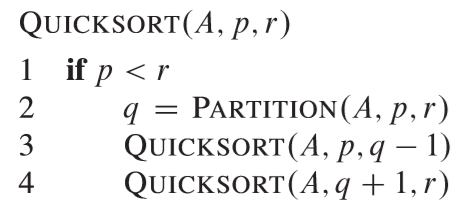
\includegraphics[width=0.9\textwidth]{figs/quicksort.png}
		\end{center}
		\column{0.1\textwidth}
		\begin{center}\textbf{\color{red}VS}
		\end{center}
		\column{0.45\textwidth}
		\begin{center}
			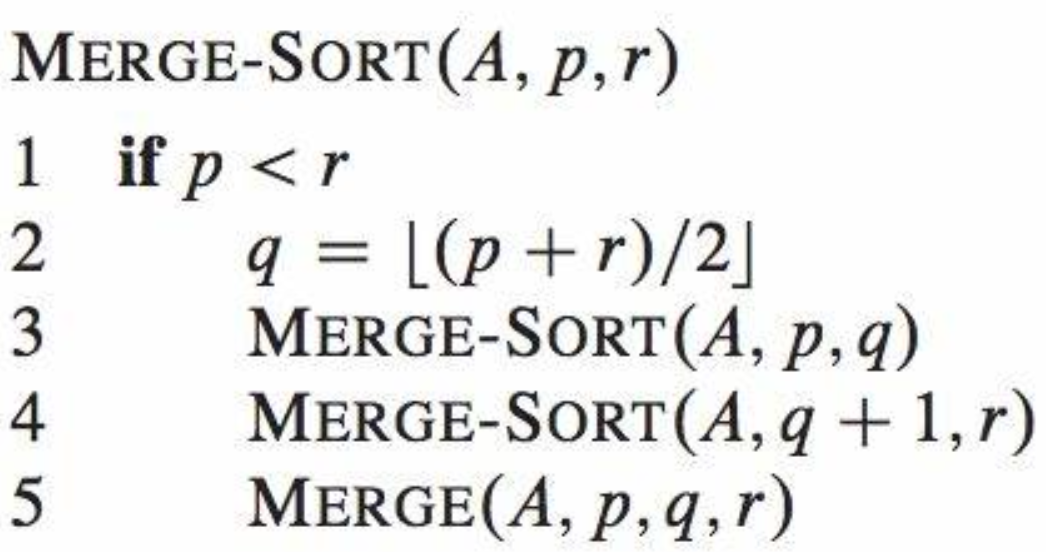
\includegraphics[width=0.9\textwidth]{figs/mergesort.png}
		\end{center}
	\end{columns}

	\end{center}
	\begin{block}{}
		\begin{description}
			\pause\item[Similarity:] both are {\color{red}\textbf{divide-and-conquer}} strategies.
			\pause\item[Difference:]  the process
			\begin{center}
				\begin{table}[]
					\centering
					\begin{tabular}{c|cc}
						\textbf{} & \textbf{QuickSort} & \textbf{MergeSort} \\\hline
						Partition    & hard               & {\color{blue}easy}               \\
						Combination   & {\color{blue}easy}                 & hard              
					\end{tabular}
				\end{table}
			\end{center}
		\end{description}
	\end{block}
\end{frame}

\begin{frame}[t]
	\frametitle{Quicksort: \textproc{Partition}}
	\begin{columns}
		
		\column{0.5\textwidth}
		\begin{block}{}
		\begin{center}
		\begin{tikzpicture}[scale=5/6]
		\node at (0,0) {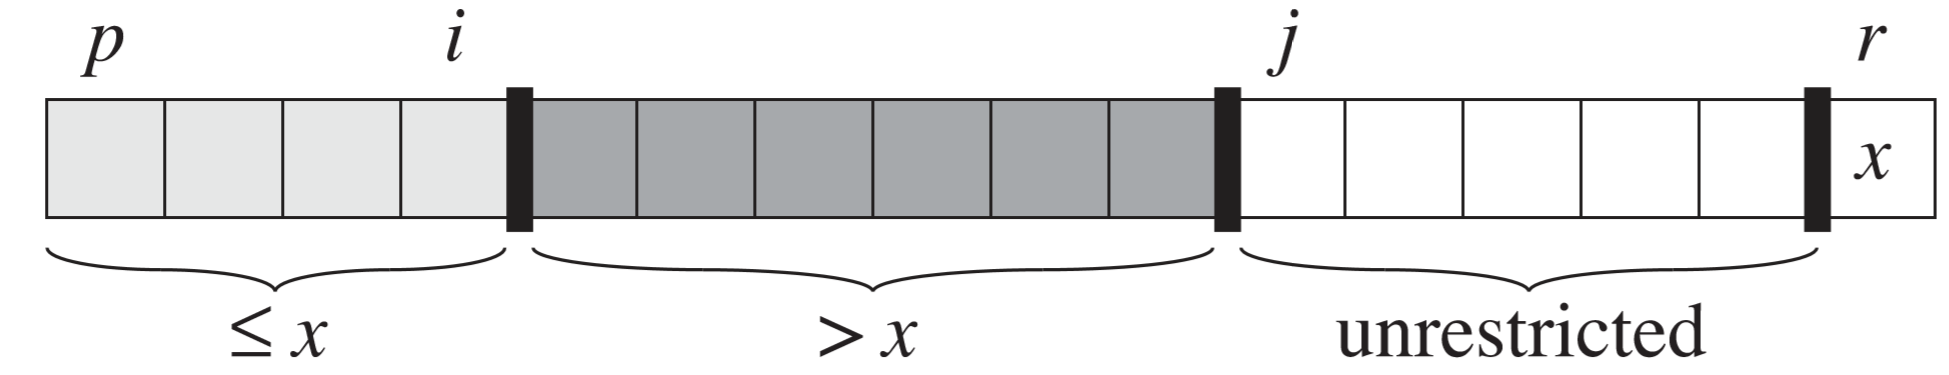
\includegraphics[width=0.9\textwidth]{figs/quicksort__partition_process.png}};
		\node (a) at(-3,0.6){ };
		\node (b) at(3.2,0.6){ };
		\node at(0.1,0.9)[color=orange]{$k$};
		\draw[decorate,decoration=brace,color=orange, line width=1pt] (a)--(b);
		\node at (0,-3) {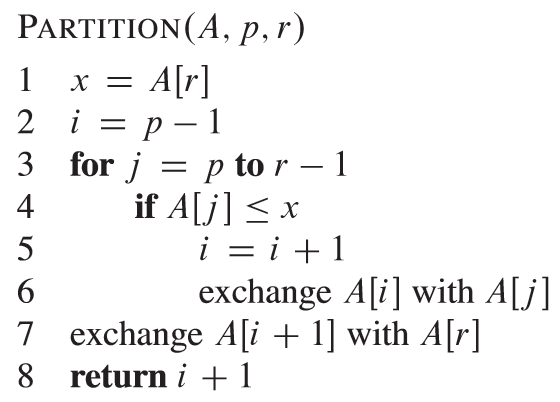
\includegraphics[width=.9\textwidth]{figs/quicksort_partition_procedure.png}};
		\onslide<2->\draw [color=red,thick](-2.5,-2.3) rectangle (-2.2,-1.8);
		\onslide<3->\draw [color=red,thick](-1.8,-2.85) rectangle (-1.5,-2.35);
		\onslide<4->\draw [color=gray,thick](-2.5,-2.35) rectangle (3.5,-4.4);
		\end{tikzpicture}
		\end{center}
	\end{block}
	
	\column{0.5\textwidth}
	\question{}{ How to prove the correctness of \textproc{Partition}?}
	\begin{block}{}
		\vspace{0.2cm}
		\onslide<4->{
		At the beginning of each iteration of the loop of lines 3-6, for any array index $k$, we have:
		
		\vspace{0.2cm}
		\fbox{	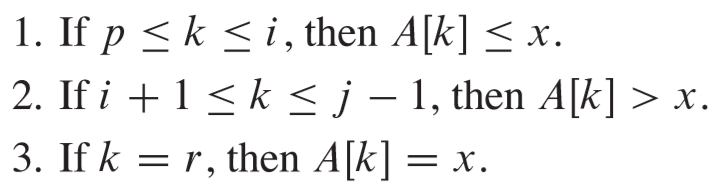
\includegraphics[width=.9\textwidth]{figs/correctness_quicksort_partition_procedure.png}
		}
	}
	\end{block}
	
	\end{columns}
\end{frame}

\begin{frame}[t]
	\frametitle{Quicksort: Time Complexity}
	\question{}{What is the time complexity of \textproc{Quicksort}?}
	\begin{center}
		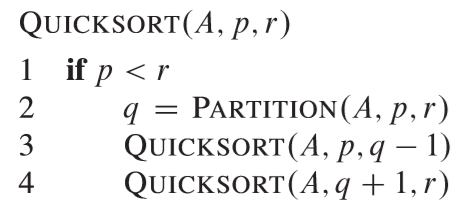
\includegraphics{figs/quicksort.png}
	\end{center}

	\begin{center}
	\pause	\begin{block}{The recurrence: $T(n)=T(n_1)+T(n_2)+cn$} where:
	\pause		\[
				\begin{array}{ll}
					n_1=q-1-p+1=q-p\\
					n_2=r-(q+1)+1=r-q\\
					n_1+n_2=r-p\\
					{\color{blue}initially}, p=1, r=n
				\end{array}
			\] 
			
\pause		$n_1,n_2$ vary and depend on 	{\color{blue}$q=\textproc{Partition}(A,p,r)$}
		\end{block}
	\end{center}
\end{frame}

\begin{frame}[t]
	\frametitle{Quicksort: Time Complexity}
	\question{}{Which factor would affect the efficiency of \textproc{Quicksort}?}
	\begin{center}
		\begin{tikzpicture}
			
			\node at (0,0) {	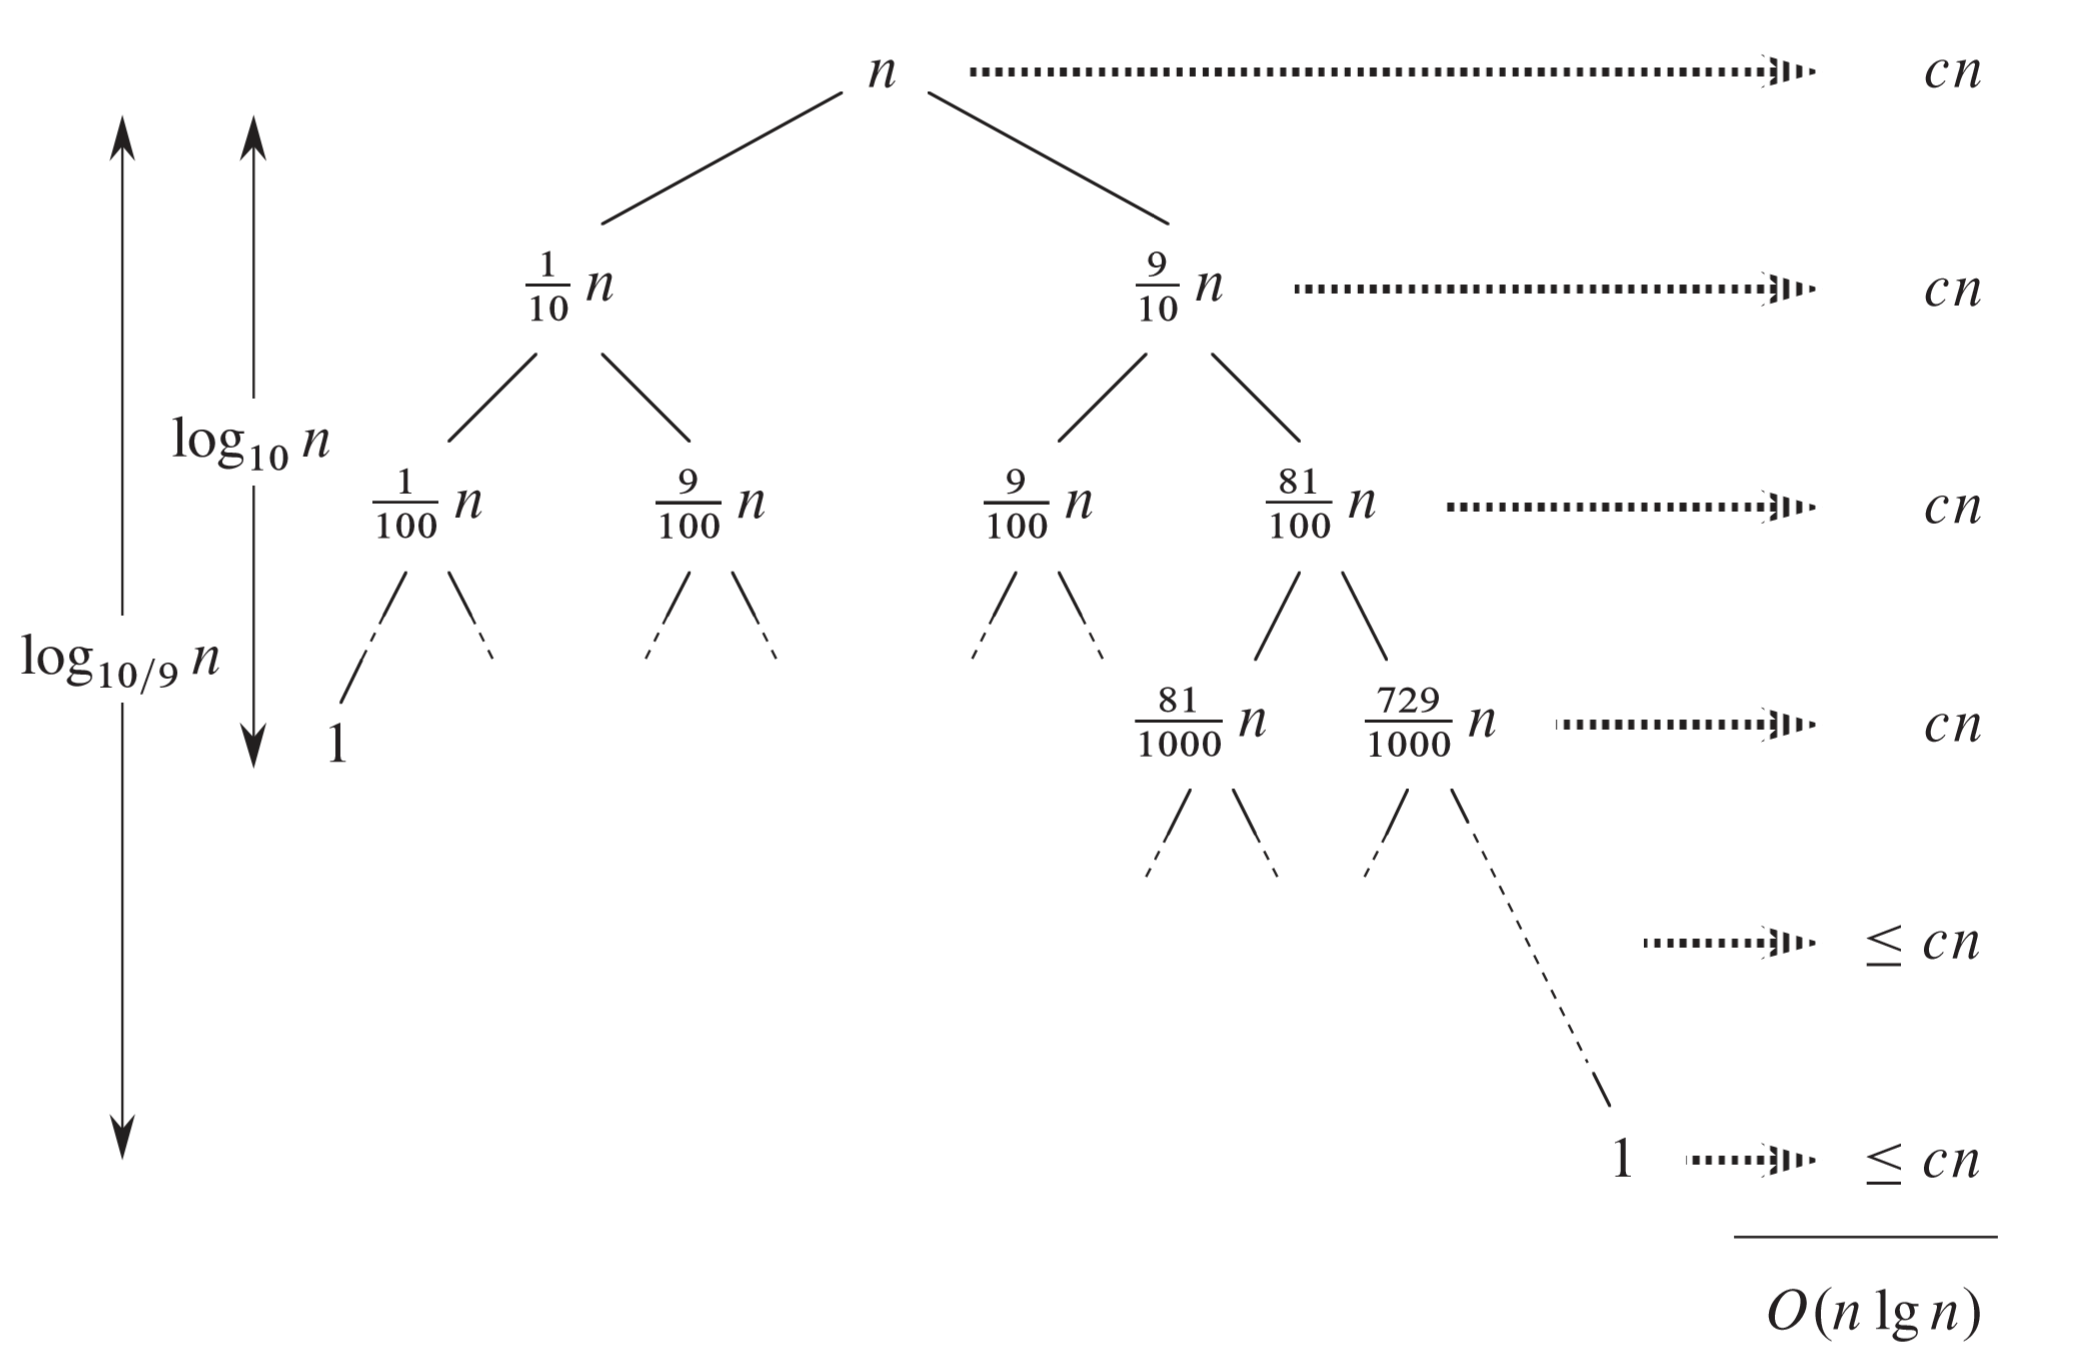
\includegraphics[height=0.7\textheight]{figs/recur_tree_quicksort.png}};
			\draw [color=red](-4.6,-0.2) rectangle (-3.6,0.2);
			\draw [color=red](-4.0,0.8) rectangle (-3.1,1.2);
			\node at(-2,3.5){\fbox{always produces a 9-to-1 split}};
			\pause\node at(-1,-2)[fill= yellow,text width=4.5cm] {the choice of {\color{blue}Pivot} would affect the tree height.};
		\end{tikzpicture}
	
	\end{center}
\end{frame}

\begin{frame}[t]
	\frametitle{Quicksort: Time Complexity}
	\question{}{Which factor would affect the efficiency of \textproc{Quicksort}?}
	\begin{center}
		\begin{tikzpicture}
		\node at (0,0) {	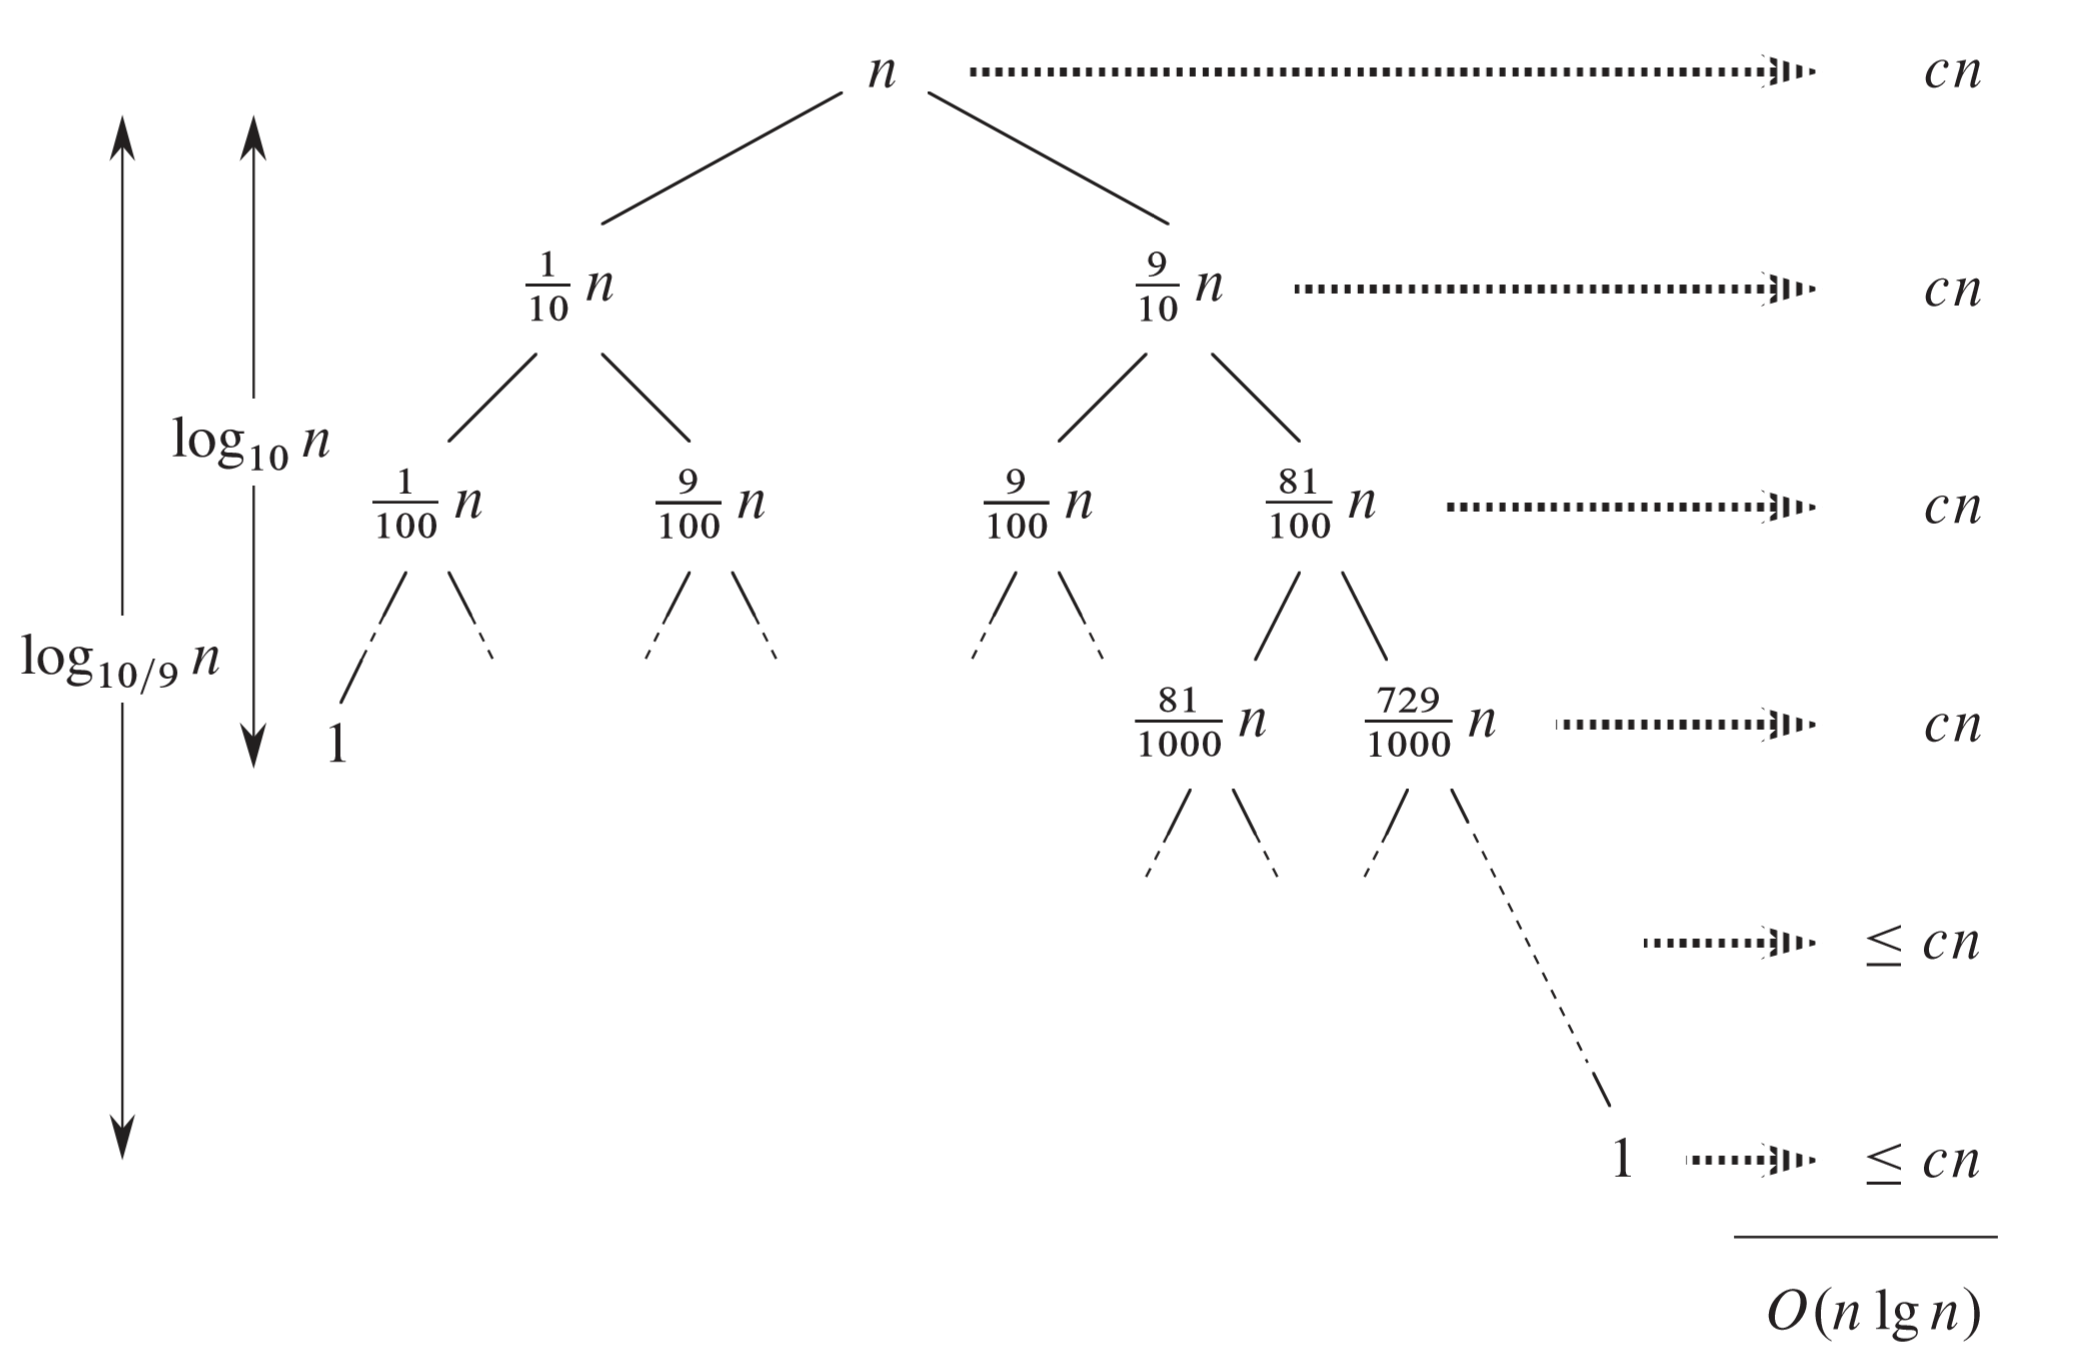
\includegraphics[height=0.7\textheight]{figs/recur_tree_quicksort.png}};
		\draw [color=red](-4.6,-0.2) rectangle (-3.6,0.2);
		\draw [color=red](-4.0,0.8) rectangle (-3.1,1.2);	
		
		\node at(-2,3.5){\fbox{always produces a 9-to-1 split}};
		\node at(-0.8,-1.8)[fill= green!30!black!30!,text width=5.8cm] {any split of \emph{\color{red}constant proportionality}\\
		\begin{itemize}
		\item  tree height: {\color{blue}$\Theta(\lg{n})$}
		\item  cost of each level: {\color{blue}$cn$}
		\item  total running time: {\color{blue}$O(n\lg{n})$}
		\end{itemize}};
		\end{tikzpicture}
		
	\end{center}
\end{frame}

\begin{frame}[t]
	\frametitle{Quicksort: Time Complexity}
	\question{}{Which factor would affect the efficiency of \textproc{Quicksort}?}
	\begin{center}
		\begin{tikzpicture}
		\node at (0,0) {	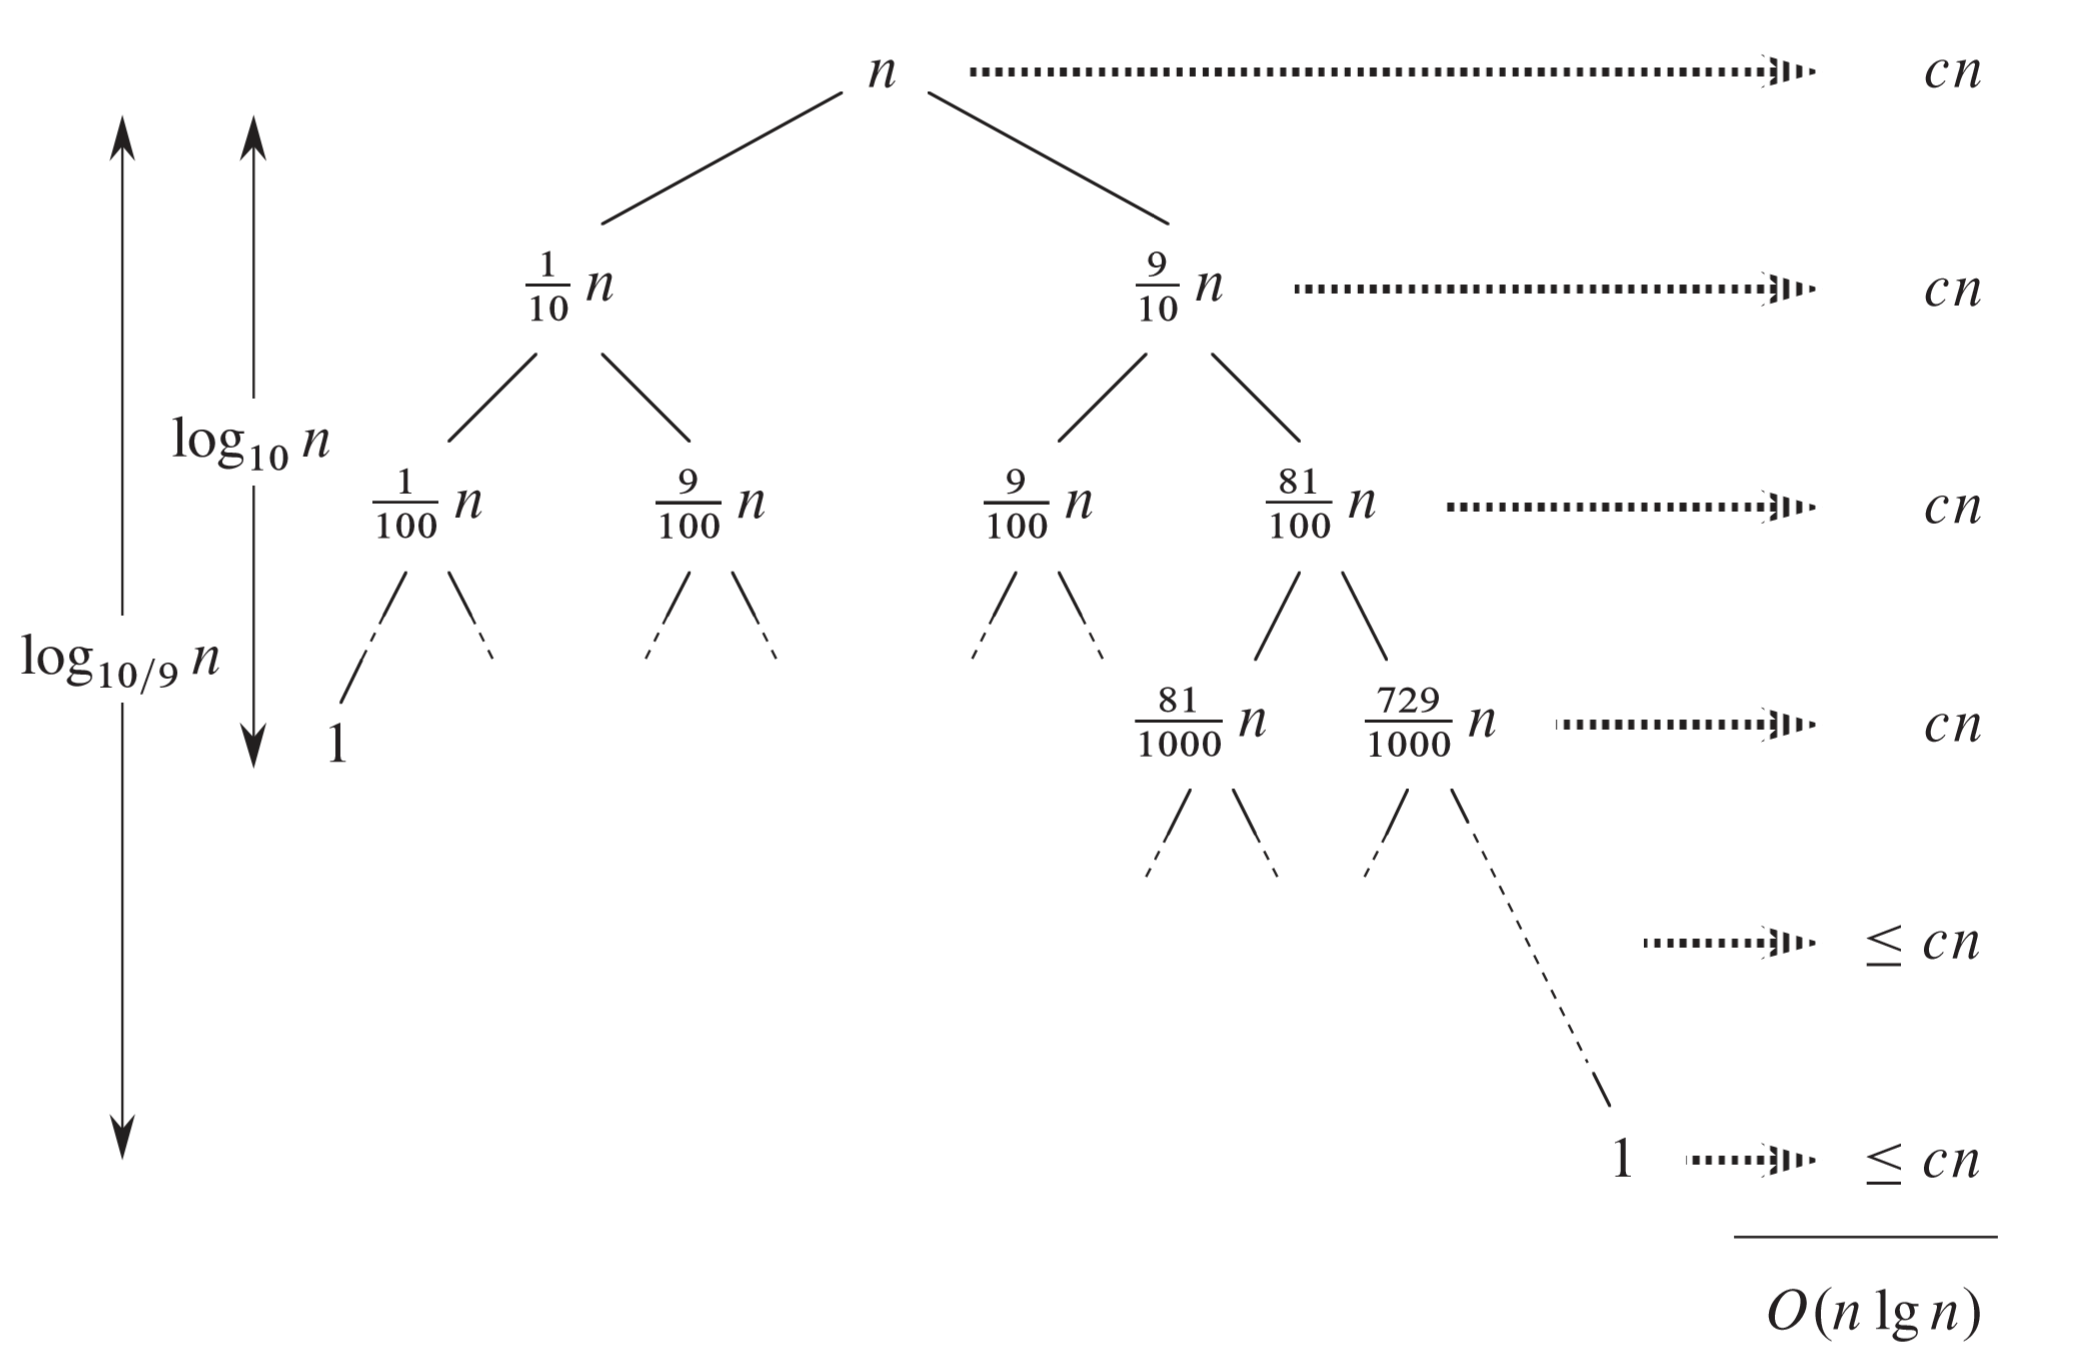
\includegraphics[height=0.7\textheight]{figs/recur_tree_quicksort.png}};
		\draw [color=red](-4.6,-0.2) rectangle (-3.6,0.2);
		\draw [color=red](-4.0,0.8) rectangle (-3.1,1.2);
		\node at(-0.8,-1.4)[fill= green!30!black!30!,text width=5.8cm] {any split of {\color{red}\xout{\emph{constant proportionality}}}\\
			What is the {\color{red}WORST CASE}?
		};
		\pause	\node at(-1.6,-2.6)[fill= blue!30!black!30!] {\color{blue}
		$T(n)=\max_{0\le q\le n-1}(T(q)+T(n-q-1))+\Theta(n)$};
		\end{tikzpicture}			
	\end{center}
\end{frame}

\begin{frame}[t]
	\frametitle{Quicksort: Time Complexity}
	\begin{block}{Worst Case: }
		\begin{center}
			$T(n)=\max_{0\le q\le n-1}(T(q)+T(n-q-1))+\Theta(n)$
		\end{center}
	\end{block}
	\question{}{When would the worst case happen?}
	
	\pause\begin{center}
		The pivot is {\color{red}always} the \textcolor{blue}{greatest} or \textcolor{blue}{smallest} element for each recursion.
	\end{center}

	\pause\begin{block}{\textbf{\color{red}Unlucky}: $T(n)=O(n^2)$ for the worst case!}
	\end{block}
	\pause\begin{block}{\textbf{\color{red}Lucky}: worst case seldom happens!}
	\end{block}
\end{frame}

\begin{frame}[t]
	\frametitle{Quicksort: Time Complexity}

	\onslide<1->\begin{block}{\textbf{\color{red}Impression \& Intuition}:\\
	}
	\begin{center}
		 Quick sort performs quite well in practice.\\\vspace{0.3cm} 
		\pause We usually obtain an $O(n\lg{n})$ execution in most cases, rather than the worst case.\\\vspace{0.3cm} 
		\pause\textbf{\LARGE\color{red}WHY?}\\
		\pause {\color{blue}\textproc{Partition} produces a mix of ``good'' and ``bad'' splits.}\\
			
		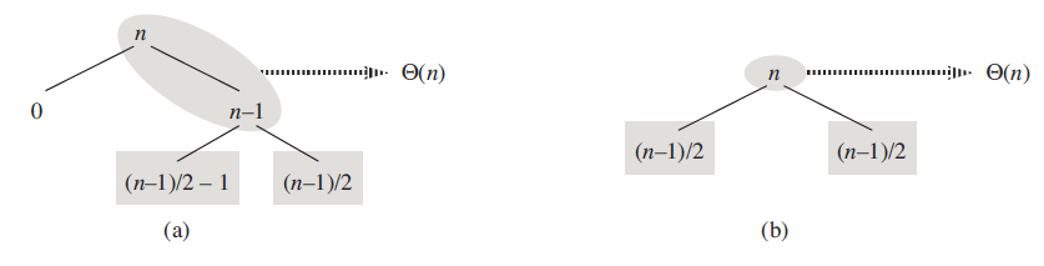
\includegraphics[height=.3\textheight]{figs/quicksort_binary_tree.png}
		
		\pause {\color{blue}$T(n)=O(n\lg{n})$}
	\end{center}
	\end{block}
\end{frame}
\begin{frame}[t]
	\frametitle{Quicksort: Time Complexity}
	\begin{block}{\textbf{\color{red}Critical operation?}}
	\begin{itemize}
		\item The key cost of Quicksort comes from {\color{blue}\textproc{Partition}}
		\item The key cost of \textproc{Partition} comes from line {\color{blue}4}.
	\end{itemize}	
	\end{block}
	\begin{center}
		\begin{columns}
			\begin{column}[T, onlytextwidth]{.45\textwidth}
				\begin{tikzpicture}
					\node at(0,0) {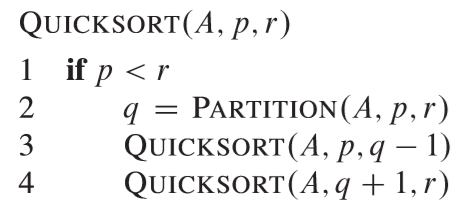
\includegraphics[height=.25\textheight]{figs/quicksort.png}};
					
					\draw [thick,color=blue] (-1.2,-0.2)--(2.2,-0.2);
				\end{tikzpicture}
			\end{column}
			\begin{column}[T, onlytextwidth]{.45\textwidth}
				\begin{tikzpicture}
					\node at(0,0){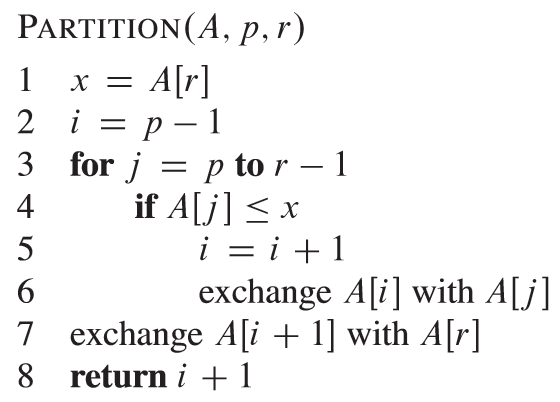
\includegraphics[height=.4\textheight]{figs/quicksort_partition_procedure.png}};
					\draw [thick,color=blue] (-1.2,-0.2)--(0.2,-0.2);
				
				\end{tikzpicture}
				
			\end{column}
		\end{columns}
	
	\end{center}
\end{frame}

\begin{frame}[t]
\frametitle{Quicksort}
\begin{center}	
	\begin{lemma}[7.1]
		Let {\color{blue}$X$} be the number of comparisons performed in line 4 of \textproc{Partition} over the entire execution of \textproc{Quicksort} on an $n$-element array. Then the running time of \textproc{Quicksort} is {\color{blue}$O(n+X)$}. 
	\end{lemma}
	\begin{proof}
		 By the discussion above, the algorithm makes at most {\color{blue}$n$} calls to \textproc{Partition}, each of which does a constant amount of work and then executes the \textbf{\color{blue}for loop}  some number of times. Each iteration of the \textbf{\color{blue}for loop}  executes line $4$.
	\end{proof}
\end{center}
\end{frame}

\subsection{Randomized Quicksort}
\begin{frame}[t]
	\frametitle{Randomized Quicksort}
	\begin{columns}
	
	\begin{column}[T, onlytextwidth]{.5\textwidth}
	\begin{block}{Randomized Quicksort}
		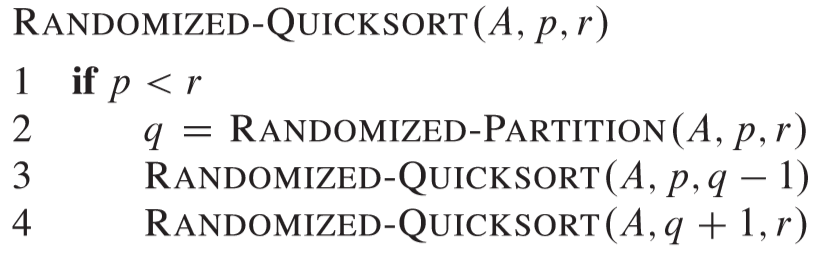
\includegraphics[height=.23\textheight]{figs/randomized-quicksort.png}
	\end{block}
	\begin{block}{\textbf{\color{red}Goal:}}
		To compute $X$, the \textbf{\color{blue}TOTAL} number of comparisons performed in \textbf{all} calls to \textproc{Partition}. 
		
		We will \textbf{NOT} attempt to analyze how many comparisons are made in  \textbf{\color{blue}EACH} call to \textproc{Partition}.
	\end{block}
	\end{column}
	\begin{column}[T, onlytextwidth]{.4\textwidth}
	\begin{block}{Randomized Partition}
	
			\begin{tikzpicture}
			\node at(0,0) {	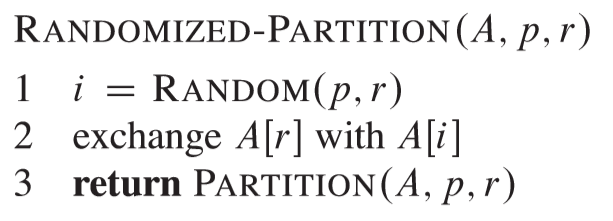
\includegraphics[height=.2\textheight]{figs/randomized-partition-procedure.png}};
			
			\draw [thick,color=blue] (-1.2,-0.7)--(2,-0.7);
			\end{tikzpicture}
			\begin{tikzpicture}
			\node at(0,0){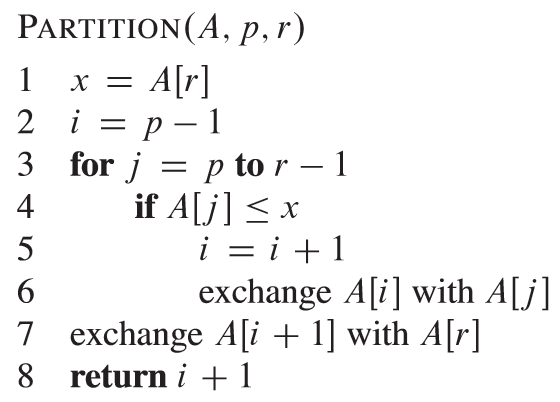
\includegraphics[height=.4\textheight]{figs/quicksort_partition_procedure.png}};
			\draw [thick,color=blue] (-1.2,-0.2)--(0.2,-0.2);
			\end{tikzpicture}
		\end{block}
	\end{column}

	\end{columns}
\end{frame}



\begin{frame}[t]
\frametitle{Randomized Quicksort: Expected Running Time}
\question{}{How to compute the expected value of X?}
		\fbox{%
			\parbox{\textwidth}{%
				\begin{center}
					$X$: the \textbf{\color{blue}TOTAL} number of comparisons performed in \textbf{all} calls to \textproc{Partition}.
				\end{center}
			}%
		}
	\begin{itemize}
		\pause\item 	We must understand \textbf{when the algorithm compares two elements of the array and when it does not}.
		\pause\item For ease of analysis, we rename the elements of the array $A$ as $\{z_1,z_2,...,z_n\}$, with $z_i$ being the $i$th smallest element. 
		\pause\item   $Z_{ij}=\{z_i,z_{i+1},...,z_j\}$: the set of elements between $z_i$ and $z_j$, inclusive. 
	\end{itemize}


\end{frame}

\begin{frame}[t]
\frametitle{Randomized Quicksort: Expected Running Time}
\question{}{When does the algorithm compare $z_i$ and $z_j$?}
	\begin{itemize}
		\item  Each pair of elements is compared \textbf{\color{blue}at most once}
		\item  Elements are compared \textbf{\color{blue}only to the pivot element}
		\item  After a particular call of \textproc{Partition} finishes, \textbf{\color{blue}the pivot element} used in that call is \textbf{\color{blue}never again} compared to any other elements. 
	\end{itemize}
\pause\begin{block}{$X_{ij}$: indicator random variables}
	\begin{center}
		\fbox{		$X_{ij}=I\{z_i \text{ is compared to } z_j\}$}
	\end{center}
\end{block}
\pause\begin{block}{Then, we have:}
	\begin{center}
		\fbox{$X=\sum_{i=1}^{n-1}{\sum_{j=i+1}^{n}{X_{ij}}}$}
	\end{center}
\end{block}
\end{frame}

\begin{frame}[t]
\frametitle{Randomized Quicksort: Expected Running Time}
\question{}{ How to compute the expected value of $X$?}
	\begin{center}
		\fbox{$E\left[ X\right] =E\left[\sum_{i=1}^{n-1}{\sum_{j=i+1}^{n}{X_{ij}}}\right] $}
	\[	
		\begin{array}{ll}
			E\left[X\right]&=E\left[\sum_{i=1}^{n-1}{\sum_{j=i+1}^{n}{X_{ij}}}\right]\\\vspace{1ex} 
			&{\color{green!80!black!80!}=\sum_{i=1}^{n-1}{\sum_{j=i+1}^{n}{E\left[X_{ij}\right]}}}\\\vspace{1ex} 
			&=\sum_{i=1}^{n-1}{\sum_{j=i+1}^{n}{\color{red}Pr\{z_i \text{ is compared to } z_j\}}}\\\vspace{1ex} 
			&{\color{green!80!black!60!}=\sum_{i=1}^{n-1}{\sum_{j=i+1}^{n}{\color{red}\frac{2}{j-i+1}}}}\\\vspace{1ex} 
			&=\sum_{i=1}^{n-1}{\sum_{k=1}^{n-i}{\frac{2}{k+1}}}\\\vspace{1ex} 
			&{\color{green!80!black!60!}<\sum_{i=1}^{n-1}{\sum_{k=1}^{n}{\frac{2}{k}}}}\\\vspace{1ex} 
			&=\sum_{i=1}^{n-1}{{O(\lg{n})}}\\\vspace{1ex} 
			&{\color{green!80!black!60!}=O(n\lg{n})}\\\vspace{1ex} 
		\end{array}
	\]
	\end{center}
\end{frame}

\begin{frame}[t]
\frametitle{Randomized Quicksort: Expected Running Time}
\question{}{What is {\color{red}$Pr\{z_i \text{ is compared to } z_j\}$}?}
\begin{block}{}
	\begin{center}
		\begin{tikzpicture}
		\node at(0,0){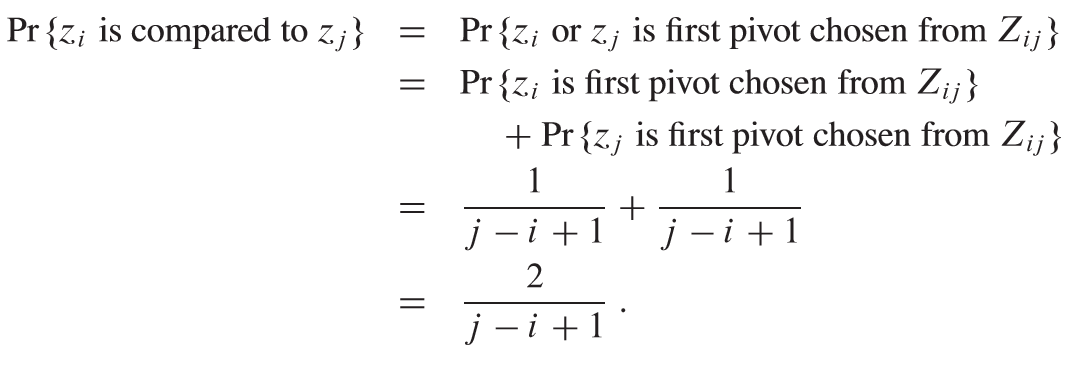
\includegraphics[width=.9\textwidth]{figs/Pr_zi_zj.png}};
		\pause\draw[color=red,thick](1.2,1.35)rectangle(2.7,1.75);
		\draw[color=red,thick](0.4,0.85)rectangle(1.9,1.25);
			
		\filldraw [color=black,fill=lightgray] (-4,-3.5)rectangle (4,-3);
		\filldraw [color=black,fill=green!20!] (-2.75,-3.5)rectangle (0.75,-3);
		\fill[ball color=blue!60] (-2.5,-3.25) circle (0.2)node[color=white]{$z_i$}; 
		\fill[ball color=blue!60] (0.5,-3.25) circle (0.2)node[color=white]{$z_j$}; 
		\draw[->,>=triangle 45,color=orange] (-3.2,-2.5)--+(0,-0.5);
		\draw[->,>=triangle 45,color=orange] (2.5,-2.5)--+(0,-0.5);
		\draw[->,>=triangle 45,color=orange] (-1,-2.5)--+(0,-0.5);
		\end{tikzpicture}
		
	\end{center}
\end{block}
\end{frame}

\begin{frame}[t]
\frametitle{Top 10 Algorithms}
\begin{block}{The 10 Algorithms with the Greatest Influence on the Development and Practice of Science and Engineering in the 20th Century}
	\begin{columns}
		\begin{column}[T, onlytextwidth]{.55\textwidth}
			\scriptsize{
			\begin{itemize}
				\item Metropolis Algorithm for Monte Carlo
				\item Simplex Method for Linear Programming
				\item Krylov Subspace Iteration Methods
				\item The Decompositional Approach to Matrix Computations
				\item The Fortran Optimizing Compiler
				\item QR Algorithm for Computing Eigenvalues
				\item \small{\textbf{\color{red}Quicksort Algorithm for Sorting}}
				\item Fast Fourier Transform
				\item Integer Relation Detection
				\item Fast Multipole Method				
			\end{itemize}
		}
		\end{column}
		\begin{column}[T, onlytextwidth]{.45\textwidth}
			\begin{center}
				
\includegraphics[width=.8\textwidth]{figs/top10.png}
				
				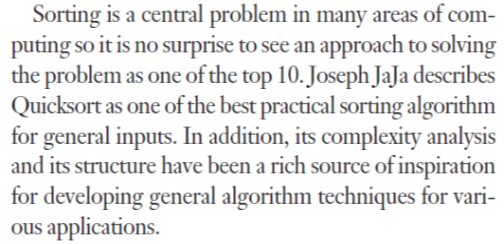
\includegraphics[width=.8\textwidth,height=0.3\textheight]{figs/top10_comments_on_quicksort.png}
			\end{center}
		\end{column}
	\end{columns}
	\begin{center}
			\fbox{\parbox{\textwidth}{\tiny{ Jack Dongarra and Francis Sullivan. 2000. Guest Editors’ Introduction: The Top 10 Algorithms. Computing in Science and Engg. 2, 1 (January 2000), 22–23. DOI:https://doi.org/10.1109/MCISE.2000.814652}}}
	\end{center}
	
\end{block}
\end{frame}
\subsection{Comparison-based Sort}
\begin{frame}
	\frametitle{Comparison-based Sort Algorithm}
	\begin{theorem}[8.1]{
		Any comparison sort algorithm requires \textbf{\color{blue}$\Omega(n\lg{n})$} comparisons in the worst case.
			
	}
	\end{theorem}
	\begin{center}
	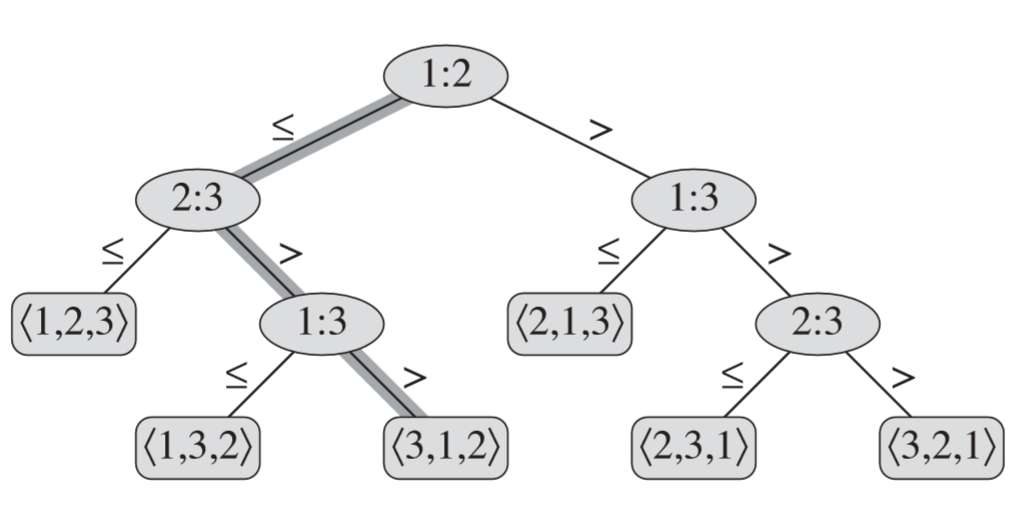
\includegraphics[width=.6\textwidth]{figs/decision_tree_comparison_based_sorting.png}
	\begin{itemize}
		\item \textbf{\color{blue}$n!$} reachable leaves, each of which corresponds to a possible permutation
		\item \textbf{\color{blue}$h$}:  the height of the decision (binary) tree
		\item $n!\le 2^h \Longrightarrow$ {\color{blue}$h\ge \lg{n!}=\Omega(n\lg{n})$}
	\end{itemize}
	\end{center}
\end{frame}

\subsection{Sorting in Linear Time}
\begin{frame}
\frametitle{Sorting in Linear Time}
\begin{itemize}
	\item Counting Sort
	\item Radix Sort
	\item Bucket Sort
\end{itemize}
\end{frame}

\begin{frame}
\frametitle{Sorting in Linear Time: Counting Sort}
\begin{center}
\begin{block}{Assumption}
	\begin{center}
	\fbox{	\parbox{0.95\textwidth}{%
			\begin{center}
			Each of the input elements is an integer in the {\color{blue}range $0$ to $k$}. 
			\end{center}
		}%
	}

$T(n)=\Theta(n+k)$, and if $k=O(n)$,  $T(n)=\Theta(n)$.
	\end{center}

\end{block}

	\begin{center}
	\begin{tikzpicture}
	\node at(-4,0){\fbox{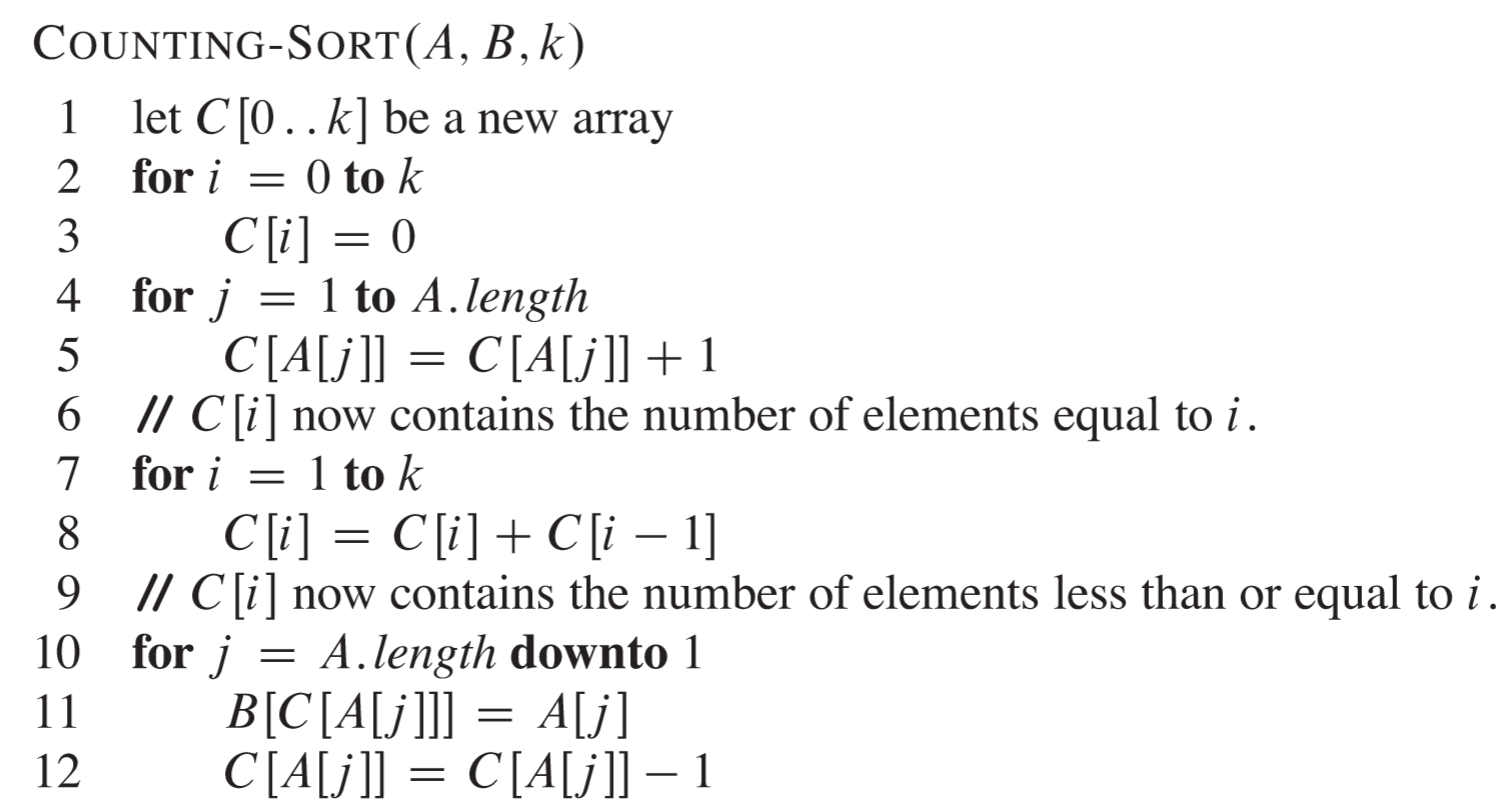
\includegraphics[width=0.6\textwidth]{figs/counting_sort_procedure.png}}};
	\node at(2,1){	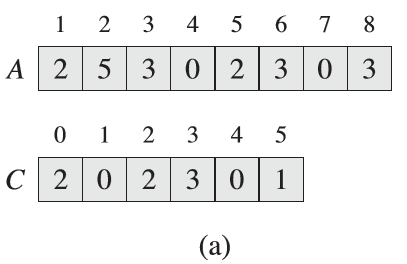
\includegraphics[width=0.3\textwidth]{figs/counting_sort_example_a.png}
	};
	\node at(1.9,-1.2){	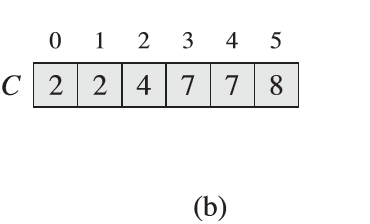
\includegraphics[width=.28\textwidth]{figs/counting_sort_example_b.png}};
	
	\onslide<2>{	\draw [color=blue](-7,-0.2) rectangle ++(5.5,0.9) node[below](a){ };
	\draw[->,color=blue](a)--++(1.7,0);
	}
	\onslide<3>{\draw [color=red](-7,-1.08) rectangle ++(6.7,0.88) node[below](b){ };
	\draw[->,color=red](b)--++(0.6,-0.4);
	}
	\onslide<4->{\draw [color=purple](-7,-1.9) rectangle ++(3,0.88) node[below,right]{\color{red}Stable};
	}
	\onslide<5->\node at (0,0.75) [fill= yellow,text width=7cm]{ \textbf{\color{red}stable:} \footnotesize{ numbers with the \textbf{\color{blue}same value} appear in the output array \textbf{\color{blue}in the same order} as they do in the input array.
	}
};
	\end{tikzpicture}
\end{center}
\end{center}
\end{frame}

\begin{frame}
\frametitle{Sorting in Linear Time: Counting Sort}
\begin{center}
	\fbox{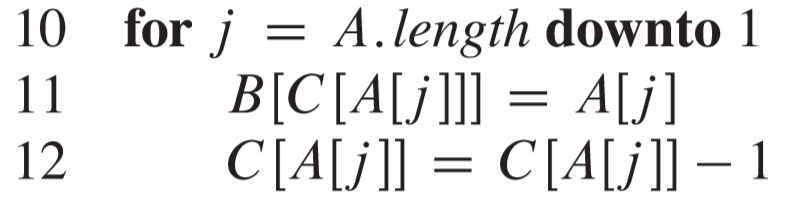
\includegraphics[width=4cm]{figs/counting_sort_procedure_output.png}}
	\begin{tikzpicture}
	\node at(-2.5,3){	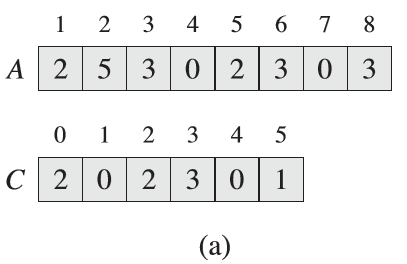
\includegraphics[width=0.3\textwidth]{figs/counting_sort_example_a.png}
	};
	\node at(2.5,3){	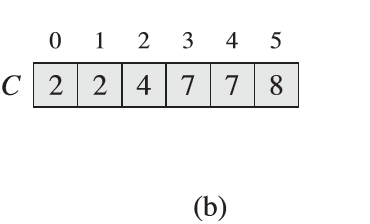
\includegraphics[width=.28\textwidth]{figs/counting_sort_example_b.png}};
	
	
	\node at(-4,0) {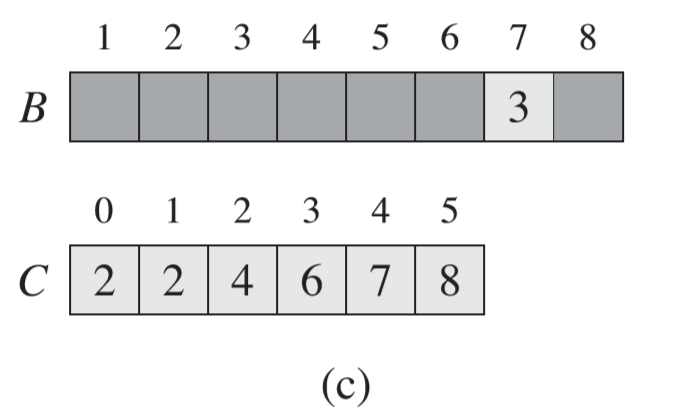
\includegraphics[width=0.31\textwidth]{figs/counting_sort_example_c.png}};
	\node at(0,0) {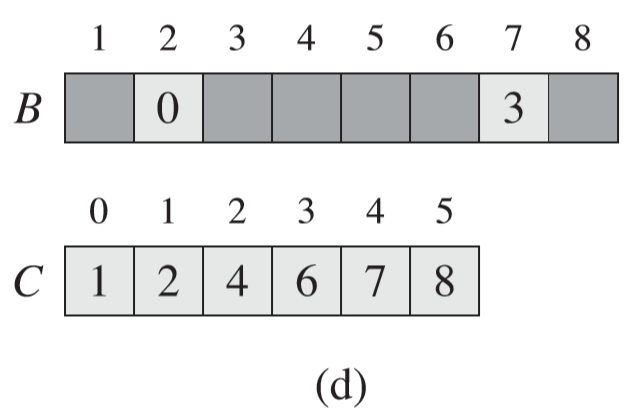
\includegraphics[width=0.3\textwidth]{figs/counting_sort_example_d.png}};
	\node at(4,0) {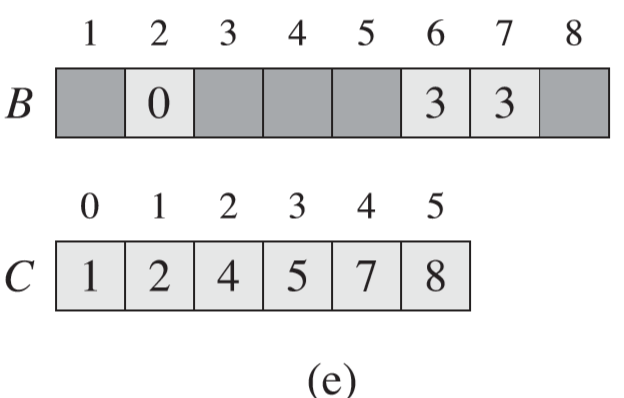
\includegraphics[width=0.3\textwidth]{figs/counting_sort_example_e.png}};
	\end{tikzpicture}
\end{center}
\end{frame}

\begin{frame}
\frametitle{Sorting in Linear Time: Radix Sort}
\begin{center}
	\begin{block}{Assumption}
		\begin{center}
			\fbox{	\parbox{0.95\textwidth}{%
					\begin{center}
						\begin{itemize}
							\item  Each element in the $n$-element array $A$ has $d$ digits, where digit $1$ is the lowest-order digit and digit $d$ is the highest-order digit.
							\item Each digit can take on up to $k$ possible values
						\end{itemize}			
					\end{center}
				}
			}
		\end{center}
		
	\end{block}
	\begin{block}{}
		\begin{center}
			\begin{tikzpicture}
			\node at (0,0) { \fbox{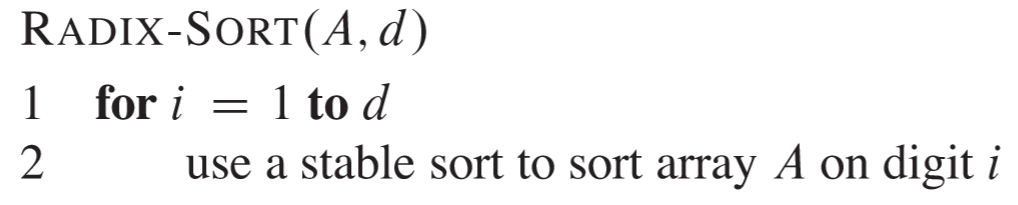
\includegraphics[width=.5\textwidth]{figs/radix_sort_procedure.png}}};
			\pause\draw [color=red,thick] (-1.5,-0.7) rectangle (0,-0.2);
			\end{tikzpicture}
			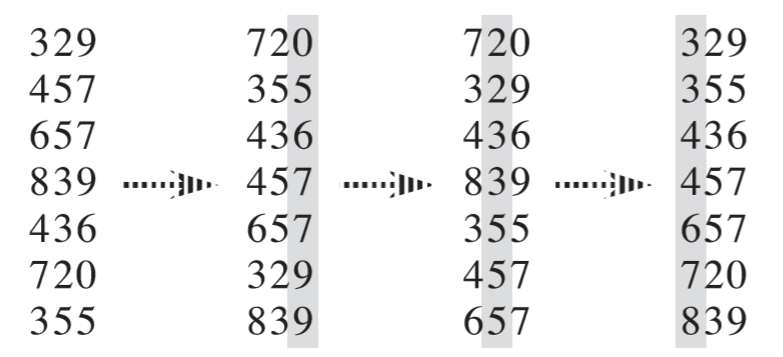
\includegraphics[width=.4\textwidth]{figs/radix_sort_example.png}
		\end{center}
	\end{block}

\end{center}
\end{frame}

\begin{frame}
\frametitle{Sorting in Linear Time: Radix Sort}
\begin{center}
	\begin{lemma}[8.3]
		Given $n$ $d$-digit numbers in which each digit can take on up to $k$ possible values, \textproc{Radix-Sort} correctly sorts these numbers in \textbf{\color{blue}$\Theta(d(n+k))$} time if the \textbf{\color{green!90!black!90!}stable sort} it uses takes \textbf{\color{green!90!black!90!}$\Theta(n+k)$} time. 
	\end{lemma}

	\begin{lemma}[8.4]
		Given $n$ $b$-bit numbers and any positive integer {\color{red}$r$}$\le b$, \textproc{Radix-Sort}  correctly sorts these numbers in $\Theta((b/r)(n+2^r))$ time if the \textbf{\color{green!90!black!90!}stable sort} it uses takes \textbf{\color{green!90!black!90!}$\Theta(n+k)$} time for inputs in the range $0$ to $k$. 
	\end{lemma}
	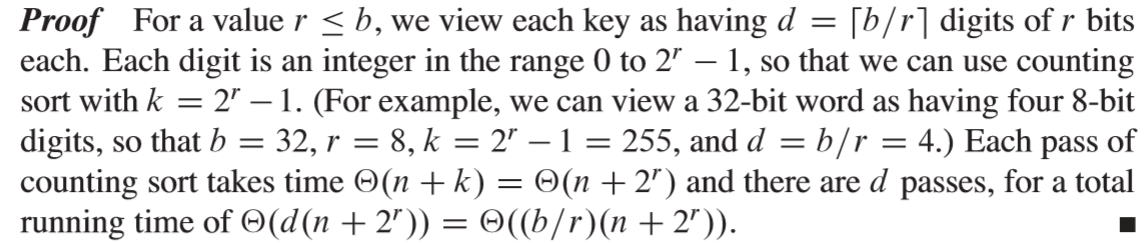
\includegraphics[width=0.9\linewidth]{figs/proof_lemma_8-4.png}
\end{center}
\end{frame}
\begin{frame}
\frametitle{Sorting in Linear Time: Bucket Sort}
\begin{center}
	\begin{block}{Assumption}

	\fbox{	\parbox{0.95\textwidth}{%
		\begin{center}
		The input is drawn from a \textbf{\color{blue}uniform distribution}
		\end{center}
	}}

	\end{block}
	\begin{center}
		\begin{tikzpicture}
		\node at (0,0) {\fbox{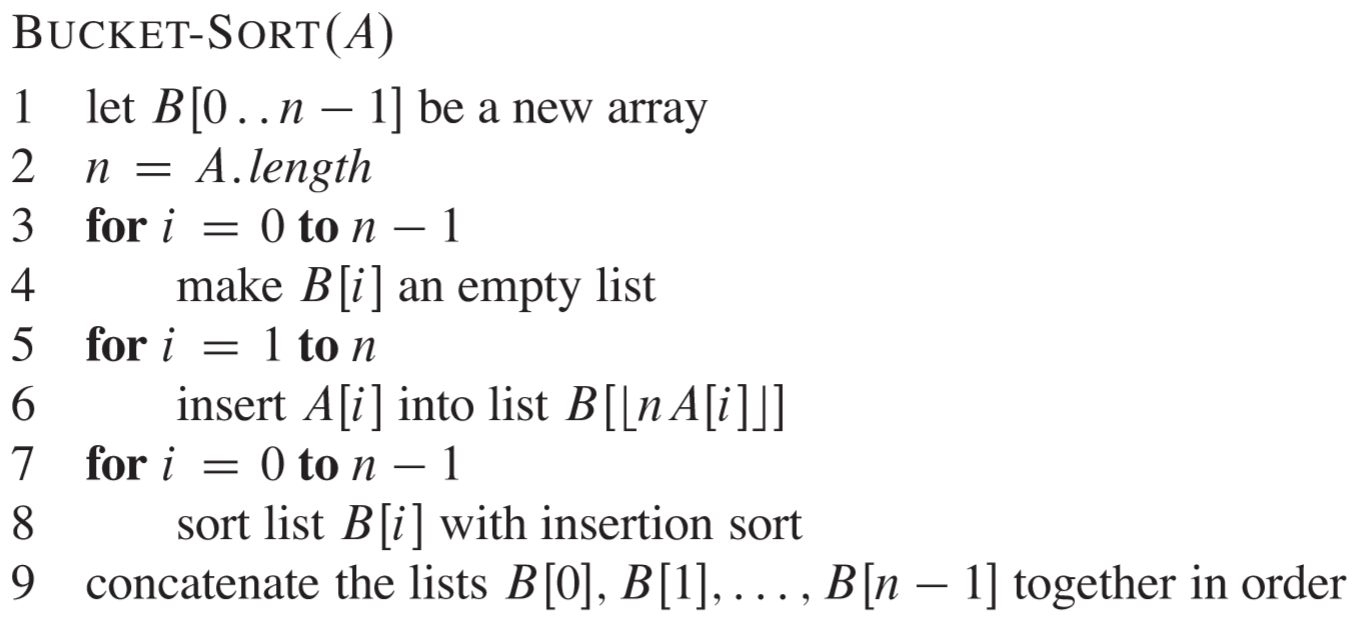
\includegraphics[width=.8\textwidth]{figs/bucket_sort_procedure.png}}};
		\node at(4,0.2) {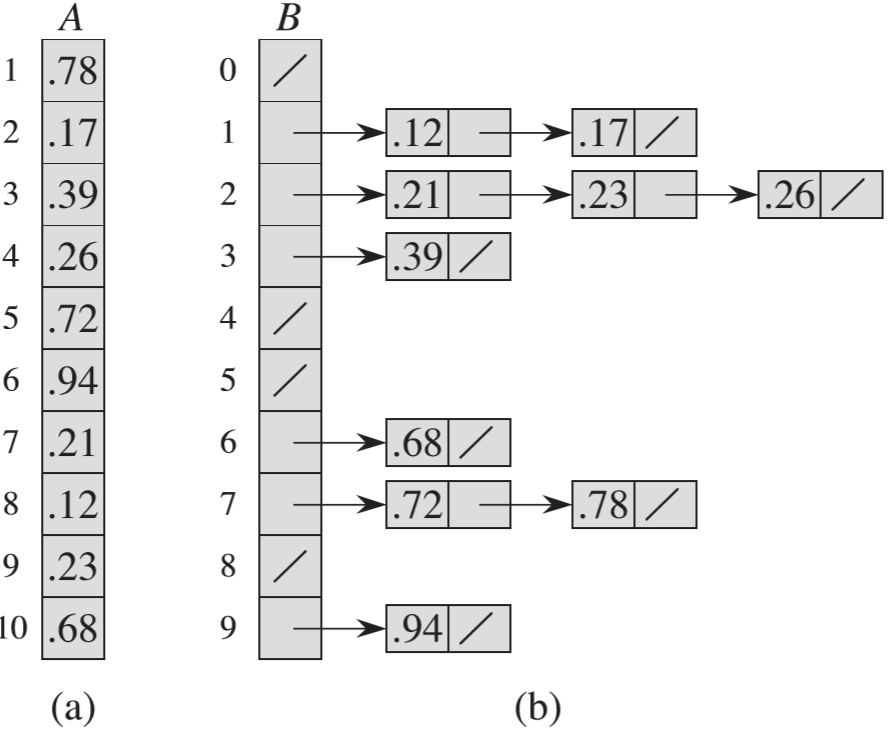
\includegraphics[width=.4\textwidth]{figs/bucket_sort_example.png}};
		\draw [color=red,thick](-1,-1.7) rectangle(1,-1.4);
		\end{tikzpicture}		
	\end{center}
\end{center}
\end{frame}


\begin{frame}
\frametitle{Sorting in Linear Time: Bucket Sort}
	\begin{center}
		\begin{tikzpicture}
		\node at (0,0) {\fbox{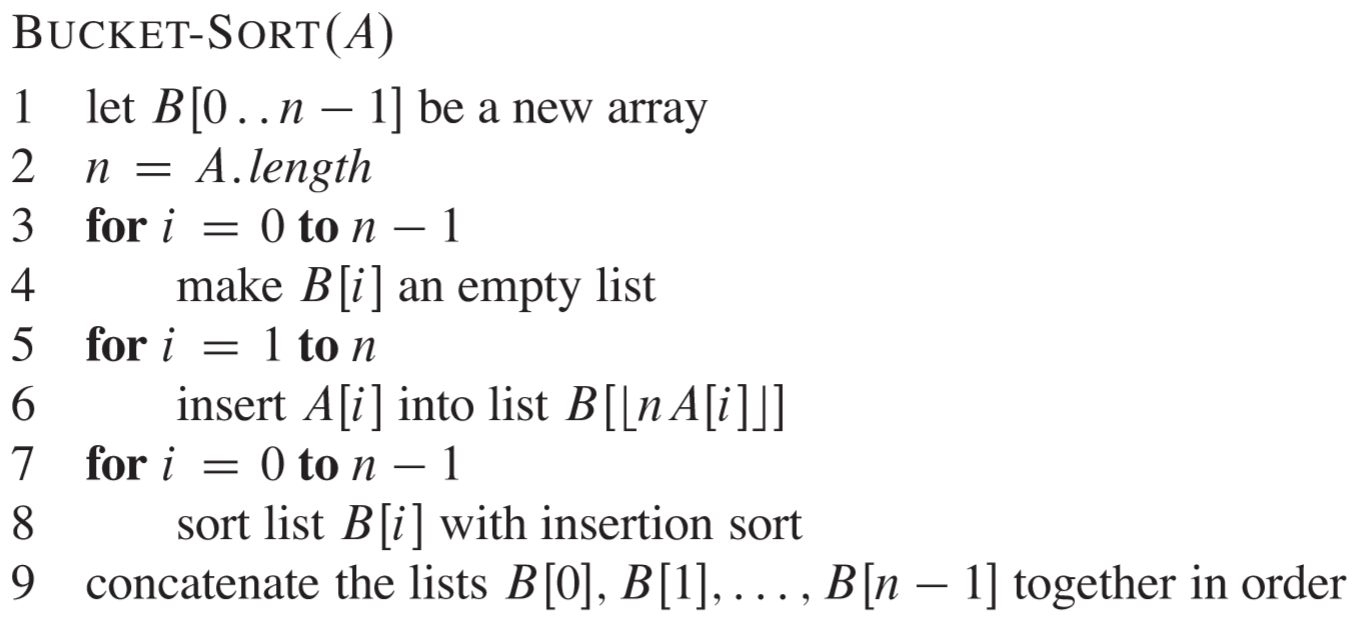
\includegraphics[width=.8\textwidth]{figs/bucket_sort_procedure.png}}};
		\draw [color=red,thick](-1,-1.7) rectangle(1,-1.4);
		\pause\node at(1.5,-1.55){\color{blue}$O(n_i^2)$};
		\pause\node at (2.5,0) {\color{blue}$T(n)=\Theta(n)+\sum\limits_{i=0}^{n-1}{O(n_i^2)}$};
		\end{tikzpicture}		
	\end{center}
\begin{itemize}
	\item All lines except line 8 take {\color{blue}$O(n)$} time in the worst case. 
	\item  {\color{blue}$n_i$}: the number of elements placed in bucket $B\left[i\right]$.
\end{itemize}
\end{frame}

\begin{frame}
\frametitle{Sorting in Linear Time: Bucket Sort}
\[
\begin{array}{ll}
E\left[T(n)\right]&=E\left[\Theta(n)+\sum\limits_{i=0}^{n-1}{O(n_i^2)}\right]\\\vspace{0.2cm}
&=\Theta(n)+\sum\limits_{i=0}^{n-1}{E\left[O(n_i^2)\right]}\\\vspace{0.2cm}
&=\Theta(n)+{\color{blue}\sum\limits_{i=0}^{n-1}{O(E\left[n_i^2\right])}}\\\vspace{0.2cm}
&=\Theta(n)
\end{array}
\]
\begin{center}
	\pause\begin{tikzpicture}
	\node at(0,0) {\fbox{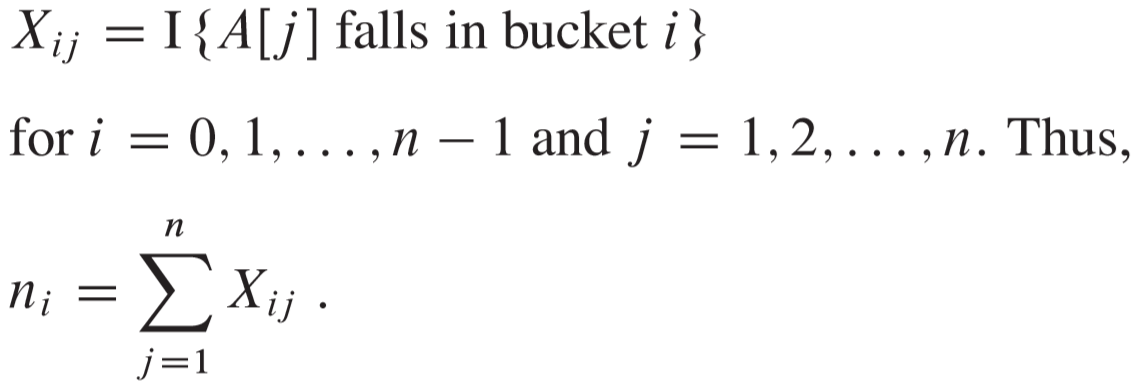
\includegraphics[width=0.5\textwidth]{figs/bucket_sort_Xij.png}}};
	\node at(6,0){\fbox{ ${\color{blue}\sum\limits_{i=0}^{n-1}{O(E\left[n_i^2\right])}=2-\frac{1}{n}}$}};
	\draw[color=blue!80!black!60!,->,>=triangle 45,line width=2pt] (3.2,0)--+(0.8,0);
	\end{tikzpicture}
	
	 	
\end{center}
\end{frame}


\section{Selection}
\subsection{Minimum and Maximum}
\begin{frame}
\frametitle{Minimum and Maximum}
\begin{center}
	\begin{problem}[Minimum or Maximum]
		Given a subset of a total-order set, find the maximum \textbf{or} minimum element of the subset. 
		\begin{itemize}
			\item requires \textbf{\color{blue}at least $n-1$} comparisons
		\end{itemize}
	\end{problem}
	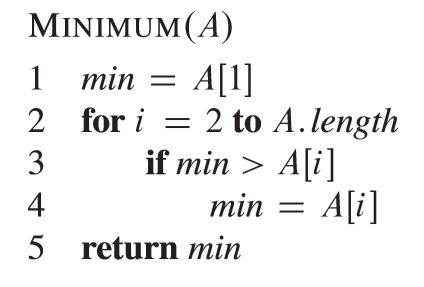
\includegraphics[width=0.4\textwidth]{figs/minimum_procedure.png}
\end{center}
\end{frame}
\begin{frame}
\frametitle{Minimum and Maximum}
\begin{center}
	
	\begin{problem}[Maximum \& minimum]
		Given a subset of a total-order set, find both the maximum \textbf{and} minimum elements of the subset. 
		\begin{itemize}
			\item does not require $2n-2$ comparisons
		\end{itemize}
	\end{problem}

\pause	\begin{proof}[A possible way for finding both maximum \& minimum]
		 \begin{itemize}
		 	\item  compare pairs of elements from the input first with each other
		 	\item then compare the smaller with the current minimum and the larger to the current maximum
		 	\item at most $3\lfloor n/2\rfloor$ comparisons
		 \end{itemize}
		
	\end{proof}
\end{center}
\end{frame}
\subsection{Selection in Expected Linear Time}
\begin{frame}
\frametitle{General Selection Problem}
\begin{problem}[General Selection]
	Given a subset of a total-order set, find the {\color{red}$i$-th} smallest element of the subset. 
\end{problem}
\end{frame}
\begin{frame}
\frametitle{Selection in Expected Linear Time
	: \textproc{Randomized-Select}}
\begin{center}
	\begin{tikzpicture}
		\node at (0,0) {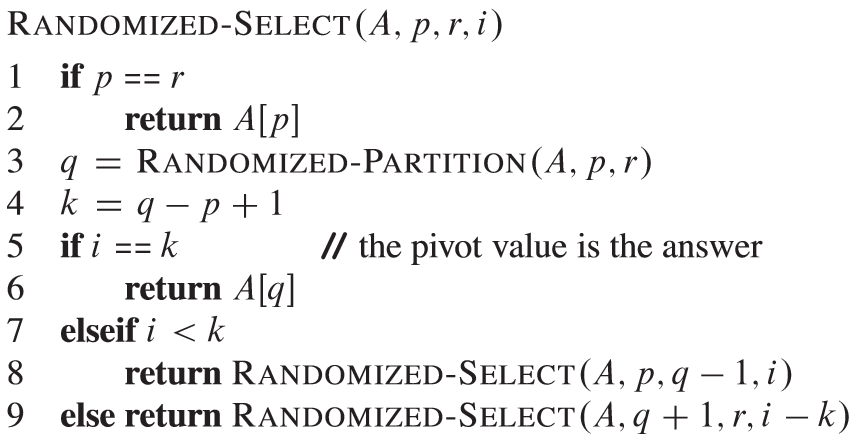
\includegraphics[width=.7\textwidth]{figs/randomized-selection-procedure.png}};
	\onslide<2->\node at (4,2) {\fbox{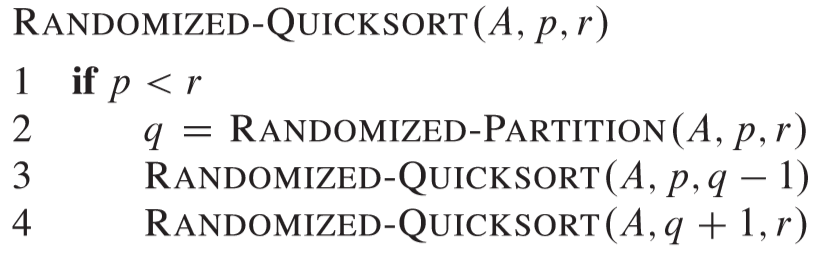
\includegraphics[width=.4\textwidth]{figs/randomized-quicksort.png}}};
		
	\end{tikzpicture}
	
	\onslide<2->{
	Similar to \textproc{Randomized-QuickSort}, but only have to handle exact one sub-problem in each step of the recursion.}

\end{center}
\end{frame}

\begin{frame}
\frametitle{\textproc{Randomized-Select}: Expected Running Time}
\question{}{What is the expected running time of \textproc{Randomized-Select}?}
\begin{center}
	\begin{columns}
		\begin{column}[T, onlytextwidth]{.6\textwidth}
			
		\pause	\begin{block}{indicator random variable \textbf{\color{red}$X_k$} :}
				\begin{itemize}
					\item	\footnotesize{
						$X_k=I\{\text{the subarray }A\left[p..q\right] \text{ has exactly }k\text{ elements}\}$	
					}
					\item assuming the elements are distinct, we have $E\left[X_k \right]=1/n $
				\end{itemize}
				
			\end{block}
		\end{column}
		\begin{column}[T, onlytextwidth]{.4\textwidth}
			\begin{tikzpicture}
			\node at (0,0) {\fbox{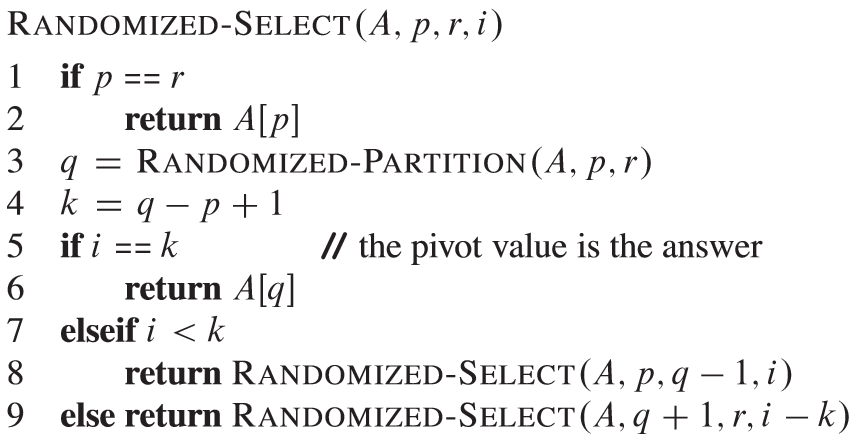
\includegraphics[width=.9\textwidth]{figs/randomized-selection-procedure.png}}};
			
			\end{tikzpicture}
		\end{column}
		
	\end{columns}
	\pause\begin{block}{$T(n)$: the running time on an input array of size $n$}
		\begin{tikzpicture}
		\node at (0,0){	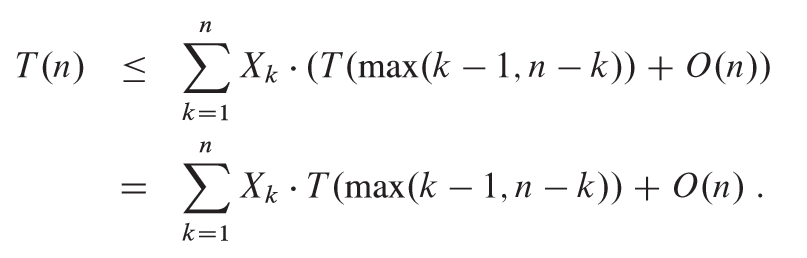
\includegraphics[width=0.6\textwidth]{figs/randomized-selection-runtime-total.PNG}};
		\pause	\draw [color=red,thick] (-2.6,0.3)rectangle ++(0.5,0.5);
		\draw [color=red,thick] (-0.8,0.3)rectangle ++(3,0.5);
		\end{tikzpicture}
	
	\end{block}
	
\end{center}
\end{frame}

\begin{frame}
\frametitle{\textproc{Randomized-Select}: Expected Running Time}

	\begin{block}{$E\left[ T(n)\right] $: the expected running time on an input array of size $n$}
		\begin{center}
		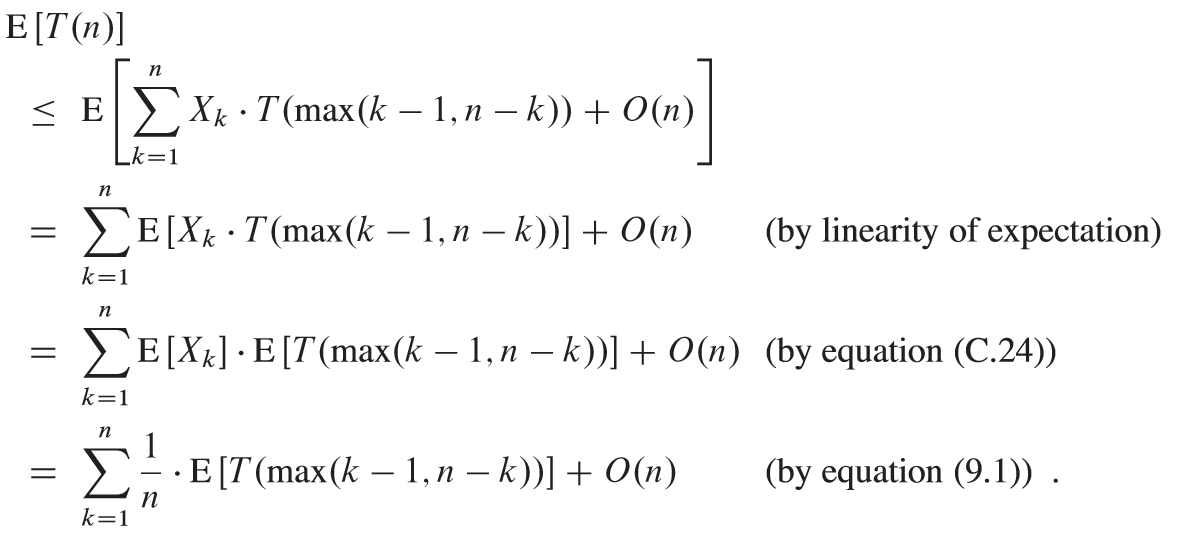
\includegraphics[width=0.8\textwidth]{figs/randomized-selection-expected-runtime-total.PNG}
		
	\pause	Then, we could prove $E\left[ T(n)\right]=O(n)$ by substitution. Assuming:
		\[
			{\color{blue} E\left[ T(n)\right]\le cn}
		\]
	
		\end{center}
	\end{block}
\end{frame}
\subsection{Selection in Worst-case Linear Time}
\begin{frame}
\frametitle{Selection in Expected Linear Time:  \textproc{Select} }

\begin{block}{\textproc{Select}}
	\begin{center}
\begin{enumerate}
	\item Divide the input array into {\color{blue}$\lceil n/5 \rceil$} groups of 5 elements each 
		\begin{itemize}
			\item at most one group made up of the remaining $n$ mod 5 elements. 
		\end{itemize} 
	\item Find the \textbf{median} of each of the {\color{blue}$\lceil n/5 \rceil$} groups with \textbf{insertion-sort}. 
	\item  Use \textproc{Select} recursively to find the \textbf{median} {\color{blue}$m^*$} of the medians found in step 2.  
	\item \textbf{\color{red}\textproc{Partition}} the input array around the \textbf{median-of-medians} $m^*$. 
	\item  Assume that {\color{blue}$m^*$} is the $k$th smallest element. If $i=k$, then return $m^*$. Otherwise, use 
\textproc{Select} recursively: 
	\begin{itemize}
		\item if $i<k$, find the $i$th smallest element on the low side
		\item if $i>k$, find the $(i-k)$th smallest element on the high side
	\end{itemize}
\end{enumerate}
	\end{center}
\end{block}
\end{frame}

\begin{frame}
\frametitle{\textproc{Select}}
\begin{block}{Step 1: Divide the input array into {\color{blue}$\lceil n/5 \rceil$} groups of 5 elements each }
	\begin{center}
		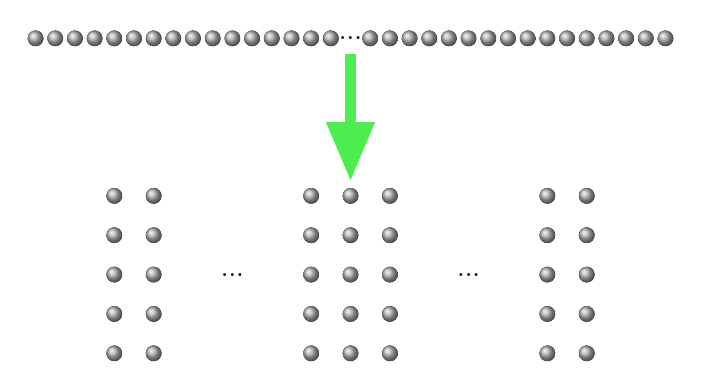
\begin{tikzpicture}
		\foreach \x in {0.25,0.5,...,4}{
				\fill[ball color=gray!60] (\x,3) circle (0.1); 
				\fill[ball color=gray!60] (0-\x,3) circle (0.1); 
		}
		\node at (0,3) {...};
		\draw[->,>=triangle 45,line width=4pt,color=green!90!black!70!] (0,2.8)--(0,1.2);
		\foreach \x in {-3,-2.5,-0.5,0,0.5,2.5,3}	
			\foreach \y in {-1,-0.5,0,0.5,1}
				\fill[ball color=gray!60] (\x,\y) circle (0.1); 
		\node at (-1.5,0) {...};
		\node at (1.5,0){...};
		\end{tikzpicture}
	\end{center}
\end{block}
\end{frame}
\begin{frame}
\frametitle{\textproc{Select}}
\begin{block}{Step 2:  Find the \textbf{median} of each of the {\color{blue}$\lceil n/5 \rceil$} groups with \textproc{insertion-sort}. }
	\begin{center}
		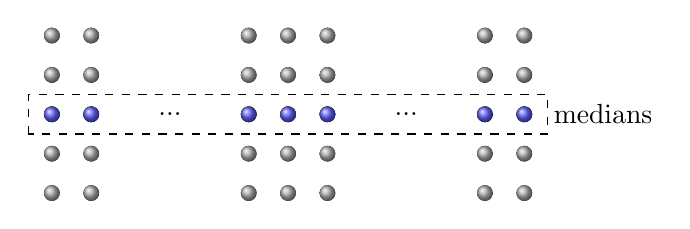
\begin{tikzpicture}
	
		\foreach \x in {-3,-2.5,-0.5,0,0.5,2.5,3}	
		\foreach \y in {-1,-0.5,0,0.5,1}
		\fill[ball color=gray!60] (\x,\y) circle (0.1); 
		\foreach \x in {-3,-2.5,-0.5,0,0.5,2.5,3}	
		\fill[ball color=blue!60] (\x,0) circle (0.1); 
		
		\node at (-1.5,0) {...};
		\node at (1.5,0){...};
		{
			\draw [dashed] (-3.3,-0.25) rectangle (3.3,0.25);
			\node at(4,0){medians};
			
		}
		\end{tikzpicture}
	\end{center}
\end{block}
\end{frame}

\begin{frame}
\frametitle{\textproc{Select}}
\begin{block}{Step 3: Use \textproc{Select} recursively to find the \textbf{median} {\color{blue}$m^*$} of the medians found in step 2. }
	\begin{center}
		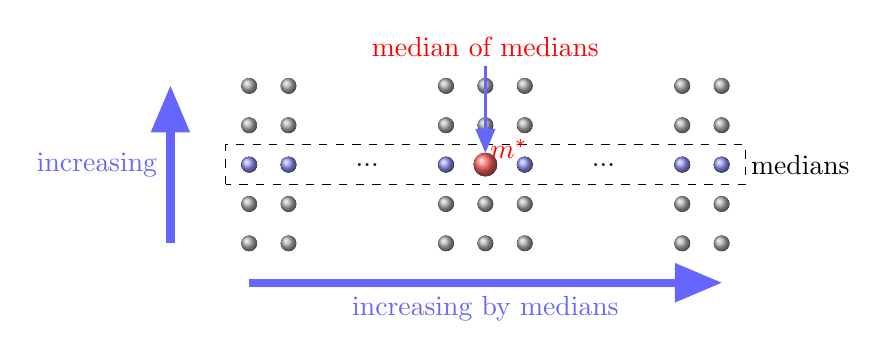
\begin{tikzpicture}

		\foreach \x in {-3,-2.5,-0.5,0,0.5,2.5,3}	
		\foreach \y in {-1,-0.5,0,0.5,1}
		\fill[ball color=gray!60] (\x,\y) circle (0.1); 
		\foreach \x in {-3,-2.5,-0.5,0.5,2.5,3}	
		\fill[ball color=blue!40] (\x,0) circle (0.1); 
		
		\node at (-1.5,0) {...};
		\node at (1.5,0){...};
		{
			\draw [dashed] (-3.3,-0.25) rectangle (3.3,0.25);
			\node at(4,0){medians};
			
		}
		\onslide<2->	{
			\fill[ball color=red!60] (0,0) circle (0.15); 
			\node (a) [color=red]at(0.3,0.2) {$m^*$};
			\node [color=red] (b) at (0,1.5){median of medians};
			\draw [->,>=triangle 45,color=blue!60,line width=1pt](b)--(0,0.15);
		}
		
		\onslide<3->{
			\draw [->,>=triangle 45,color=blue!60, line width=3pt](-4,-1)--node[left]{increasing}(-4,1) ;
			\draw [->,>=triangle 45,color=blue!60,line width=3pt](-3,-1.5)--node[below]{increasing by medians}(3,-1.5) ; 
		}
			
	
	
	
		\end{tikzpicture}
		
	\end{center}
\end{block}
\end{frame}
\begin{frame}
\frametitle{\textproc{Select}}
\begin{block}{Step 4: \textproc{Partition} the input array around $m^*$.}
	\begin{center}
		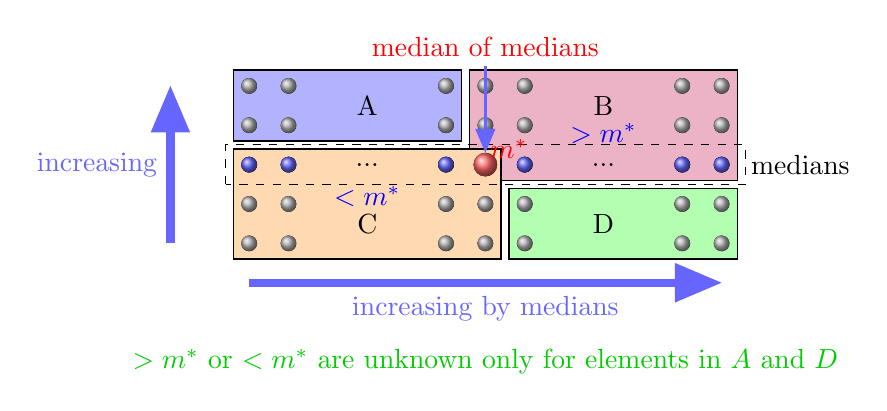
\begin{tikzpicture}
		{
			\filldraw [fill=blue!30,draw=black,line width=0.5pt] (-3.2,0.3) rectangle (-0.3,1.2); 
			
			\filldraw [fill=green!30,draw=black,line width=0.5pt] (0.3,-1.2) rectangle (3.2,-0.3); 
			\filldraw [fill=purple!30,draw=black,line width=0.5pt] (-0.2,-0.2) rectangle (3.2, 1.2); 
			\filldraw [fill=orange!30,draw=black,line width=0.5pt] (-3.2,-1.2) rectangle (0.2,0.2); 
		}
		\foreach \x in {-3,-2.5,-0.5,0,0.5,2.5,3}	
		\foreach \y in {-1,-0.5,0,0.5,1}
		\fill[ball color=gray!60] (\x,\y) circle (0.1); 
		\foreach \x in {-3,-2.5,-0.5,0.5,2.5,3}	
		\fill[ball color=blue!60] (\x,0) circle (0.1); 
		
		\node at (-1.5,0) {...};
		\node at (1.5,0){...};
		{
			\draw [dashed] (-3.3,-0.25) rectangle (3.3,0.25);
			\node at(4,0){medians};
			
		}
		{
			\fill[ball color=red!60] (0,0) circle (0.15); 
			\node (a) [color=red]at(0.3,0.2) {$m^*$};
			\node [color=red] (b) at (0,1.5){median of medians};
			\draw [->,>=triangle 45,color=blue!60,line width=1pt](b)--(0,0.15);
		}
		
		{
			\draw [->,>=triangle 45,color=blue!60, line width=3pt](-4,-1)--node[left]{increasing}(-4,1) ;
			\draw [->,>=triangle 45,color=blue!60,line width=3pt](-3,-1.5)--node[below]{increasing by medians}(3,-1.5) ; 
		}
		
		
		{
			\node at(-1.5,0.75){A};
			\node at(-1.5,-0.75){C};
			\node at(1.5,0.75){B};
			\node at(1.5,-0.75){D};
		}
		{
			\node [color=blue]at(-1.5,-0.4) {$<m^*$};
			\node [color=blue]at(1.5,0.4) {$>m^*$};
		}
		\pause{
			\node [color=green!80!black]at (0,-2.5){$>m^*$ or $<m^*$ are unknown only for elements in $A$ and $D$};
			
		}
		\end{tikzpicture}

	\end{center}
\end{block}
\end{frame}

\begin{frame}
\frametitle{\textproc{Select}}
\begin{block}{Step 5: Assume that {\color{blue}$m^*$} is the $k$th smallest element. 
		\begin{itemize}
			\item If $i=k$, then return $m^*$. 
			\item Otherwise, use \textproc{Select} recursively: 
			\begin{itemize}
				\item if $i<k$, find the $i$th smallest element on the low side
				\item if $i>k$, find the $(i-k)$th smallest element on the high side
			\end{itemize}
		\end{itemize}
	}
	\begin{center}
		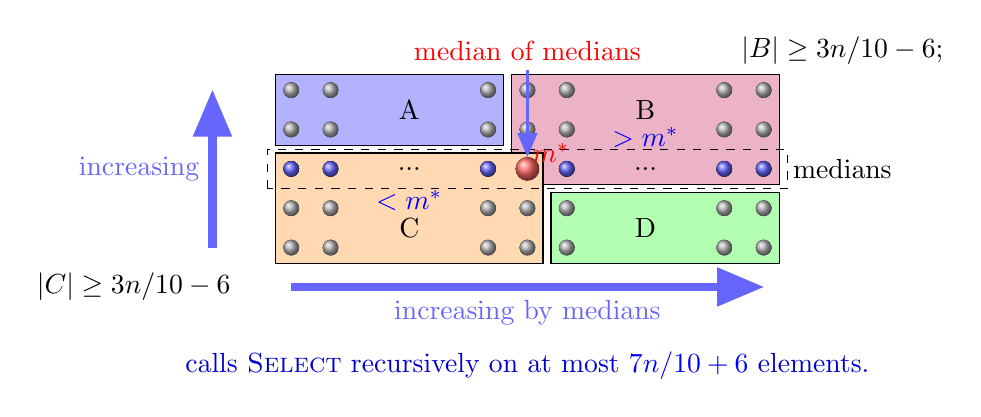
\begin{tikzpicture}
		{
			\filldraw [fill=blue!30,draw=black,line width=0.5pt] (-3.2,0.3) rectangle (-0.3,1.2); 
			
			\filldraw [fill=green!30,draw=black,line width=0.5pt] (0.3,-1.2) rectangle (3.2,-0.3); 
			\filldraw [fill=purple!30,draw=black,line width=0.5pt] (-0.2,-0.2) rectangle (3.2, 1.2); 
			\filldraw [fill=orange!30,draw=black,line width=0.5pt] (-3.2,-1.2) rectangle (0.2,0.2); 
		}
		\foreach \x in {-3,-2.5,-0.5,0,0.5,2.5,3}	
		\foreach \y in {-1,-0.5,0,0.5,1}
		\fill[ball color=gray!60] (\x,\y) circle (0.1); 
		\foreach \x in {-3,-2.5,-0.5,0.5,2.5,3}	
		\fill[ball color=blue!60] (\x,0) circle (0.1); 
		
		\node at (-1.5,0) {...};
		\node at (1.5,0){...};
		{
			\draw [dashed] (-3.3,-0.25) rectangle (3.3,0.25);
			\node at(4,0){medians};
			
		}
		{
			\fill[ball color=red!60] (0,0) circle (0.15); 
			\node (a) [color=red]at(0.3,0.2) {$m^*$};
			\node [color=red] (b) at (0,1.5){median of medians};
			\draw [->,>=triangle 45,color=blue!60,line width=1pt](b)--(0,0.15);
		}
		
		{
			\draw [->,>=triangle 45,color=blue!60, line width=3pt](-4,-1)--node[left]{increasing}(-4,1) ;
			\draw [->,>=triangle 45,color=blue!60,line width=3pt](-3,-1.5)--node[below]{increasing by medians}(3,-1.5) ; 
		}
		
		
		{
			\node at(-1.5,0.75){A};
			\node at(-1.5,-0.75){C};
			\node at(1.5,0.75){B};
			\node at(1.5,-0.75){D};
		}
		{
			\node [color=blue]at(-1.5,-0.4) {$<m^*$};
			\node [color=blue]at(1.5,0.4) {$>m^*$};
		}
	
		\pause	{
			\node at (4,1.5){$|B|\ge 3n/10-6$;};
			\node at (-5,-1.5){ $|C|\ge 3n/10-6$};
		}
		\pause 	\node [color=blue!80!black]at (0,-2.5){calls \textproc{Select} recursively on at most {\color{blue}$7n/10+6$} elements. };
		\end{tikzpicture}

	\end{center}
\end{block}
\end{frame}

\begin{frame}
\frametitle{The \textproc{Select} algorithm: Running Time in Worst-case}
\begin{block}{Counting the total number of comparisons}
	\begin{center}
		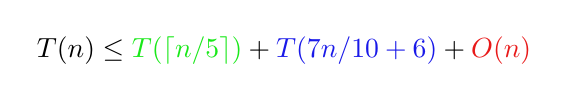
\begin{tikzpicture}
			\node at (0,0){$T(n)\le{\color{green!90!black!90!}T(\lceil n/5\rceil)}+{\color{blue!90!black!90!}T(7n/10+6)}+{\color{red!90!black!90!}O(n)}$};
		\end{tikzpicture}
		\begin{itemize}
			\item {\color{green!90!black!90!}$T(\lceil n/5\rceil)$}: find the median of the medians
			\item {\color{blue!90!black!90!}$T(7n/10+6)$}: maximum cost for   calling \textproc{Select} recursively.
			\item {\color{red!90!black!90!}$O(n)$}:
			\begin{itemize}
				\item divide the input array into  5-elements groups
				\item find medians of all 5-elements groups, about $6*\lceil n/5\rceil$
				\item \textproc{Partition} with the pivot $m^*$
			\end{itemize}
		\end{itemize}
	\end{center}
\end{block}
\begin{block}{We could show that the running time {\color{red}$T(n)=O(n)$} by substitution}
\end{block}
\end{frame}
\begin{frame}
	\begin{block}{
		\begin{center}
		{\huge
			Thank You!
			
			\textcolor[rgb]{1,0,0}	{Questions?}
		}
		\end{center}
	}
	\end{block}
	\begin{block}{}
		\begin{center}
		
			Office 819
			
			majun@nju.edu.cn
		\end{center}
	\end{block}
	\end{frame}
\end{document}